% Copyright (c) 2021-2023 Eclipse Arrowhead Project
%
% This program and the accompanying materials are made available under the
% terms of the Eclipse Public License 2.0 which is available at
% http://www.eclipse.org/legal/epl-2.0.
%
% SPDX-License-Identifier: EPL-2.0

\documentclass[a4paper]{arrowhead}

\usepackage[yyyymmdd]{datetime}
\usepackage{enumitem}
\usepackage{etoolbox}
\usepackage[utf8]{inputenc}
\usepackage{multirow}

\renewcommand{\dateseparator}{-}

\begin{document}

%% Arrowhead Document Properties
\ArrowheadTitle{Concepts Reference}
\ArrowheadType{Framework Description}
\ArrowheadTypeShort{FD}
\ArrowheadVersion{0.3}
\ArrowheadDate{\today}
\ArrowheadAuthor{Emanuel Palm and Jerker Delsing}
\ArrowheadOrganization{Eclipse Arrowhead}
\ArrowheadStatus{Proposal}
\ArrowheadContact{emanuel.palm@pinterop.se}
\ArrowheadAbstract{
  This document provides authoritative definitions for the most fundamental concepts of relevance to \textit{Eclipse Arrowhead}, a framework designed to facilitate the effective creation of service-oriented automation systems.
  It is meant to serve as foundation for other documents with relevance to the framework, providing a precise vocabulary untied to any specific practices or technologies.
  It does not contain any architectural patterns or definitions, which means that it, by itself, is not a sufficient foundation for designing Arrowhead systems.
  While its definitions are presented as a model, the document does not endorse any particular modeling language.
}
\ArrowheadFooter{\href{www.arrowhead.eu}{www.arrowhead.eu}}
\ArrowheadSetup
%%

%% Custom Document Commands
\newcommand{\GlossaryHyperRef}[2]{{\color{ArrowheadDarkBlue}\hyperref[sec:glossary:#1]{#2}}}
\newcommand{\GlossaryNameRef}[1]{{\color{ArrowheadDarkBlue}\nameref{sec:glossary:#1}}}
%%

%% Front Page
\ArrowheadFrontPage
%%

%% Table of Contents
\tableofcontents
\newpage
%%

\section{Introduction}
\label{sec:introduction}
% Copyright (c) 2021 Eclipse Arrowhead Project
%
% This program and the accompanying materials are made available under the
% terms of the Eclipse Public License 2.0 which is available at
% http://www.eclipse.org/legal/epl-2.0.
%
% SPDX-License-Identifier: EPL-2.0

We expect the automation systems of today to keep becoming more and more computerized, digitized and interconnected.
By this we mean that more aspects of and surrounding automation machines will be handled by computers, more information will be made available to those computers and, finally, comparatively more such computers will be given the opportunity to collect, communicate and act on that information.
Manufacturing, transportation, energy distribution, medicine, recycling, as well as all other industrial sectors concerned with automation we believe will be affected by this development.
It will lead to increased automation efficiency and flexibility, as machines become able to perform more of the work traditionally assigned to humans.
However, it will also lead to new magnitudes of complexity, not the least because of the renewed incentive to use more and more of these highly communicative machines.

The \GlossaryHyperRef{framework-arrowhead}{\textit{Arrowhead framework}} is designed to address this explosion of complexity.
It provides a foundation for \GlossaryHyperRef{communication-service-oriented}{\textit{service-oriented communication}} \cite{mackenzie2006reference} between automation systems and other computers, such that interoperability, security, safety, performance, and other major concerns can be addressed efficiently and effectively.
It notably allows for \GlossaryHyperRef{system}{system} \GlossaryHyperRef{capability}{capabilities} to be \GlossaryHyperRef{description}{described}, shared and exploited dynamically by communicating \GlossaryHyperRef{device}{devices}.

In this document, we, the Eclipse Arrowhead project, present an authoritative set of concept definitions, meant to serve as the fundamental language for discussions about and the modeling of Arrowhead-based system \GlossaryHyperRef{design}{designs}.
These definitions exist to help mitigate compatibility and consistency issues in \GlossaryHyperRef{software}{software}, tooling, \GlossaryHyperRef{model}{models}, documentation and all other things of relevance to the Arrowhead framework.

\subsection{Primary Audiences}
\label{sec:introduction:audiences}

This document is being written and maintained for all who need precise and rigorous definitions of important Arrowhead concepts, which we understand to likely include the following groups:

\begin{itemize}
\item \GlossaryHyperRef{developer}{Developers} of Arrowhead systems.
\item \GlossaryHyperRef{researcher}{Researchers} concerned with analyzing or refining the Arrowhead framework or Arrowhead systems.
\item \GlossaryHyperRef{builder}{Builders}, \GlossaryHyperRef{maintainer}{maintainers} and \GlossaryHyperRef{operator}{operators} of Arrowhead systems.
\item \GlossaryHyperRef{acquirer}{Acquirers}, \GlossaryHyperRef{owner}{owners} and \GlossaryHyperRef{supplier}{suppliers} of Arrowhead systems.
\item Advanced \GlossaryHyperRef{user}{users} of Arrowhead systems.
\end{itemize}

\subsection{Scope}
\label{sec:introduction:scope}

This document is intended to clearly define all technical concepts of fundamental importance to the Arrowhead framework.
It does not specify how Arrowhead-based automation systems ought to be designed.
This makes its purpose analogous to that of a dictionary.
Dictionaries define words.
They may give examples of how certain words may be used, but they do not require that those words be used for any particular purposes.
This document provides an Arrowhead vocabulary other documents or models may use to express software-centric automation system designs.

The concepts presented here are meant to be useful as a resource for advanced Arrowhead framework learners, as well as to serve as foundation for other documentation and modeling efforts.
This document does \textit{not} define an Arrowhead profile for SysML \cite{omg2019sysml}, or any other modeling language.
For those interested in using this document for software-architectural purposes, a description of how it can be used as a \GlossaryHyperRef{modelmeta}{metamodel} in the context of an ISO/IEC/IEEE 42010 \GlossaryHyperRef{kind-model}{model kind} is provided in Section \ref{sec:conformance:iso42010}.

\newpage

\subsection{Notational Conventions}
\label{sec:introduction:conventions}

The following conventions regarding diagrams depicting graphs, references and requirements are adhered to throughout this document.

\subsubsection{Graph Diagrams}

A box with a solid border and a name inside it denotes a named \GlossaryHyperRef{entity}{entity}, useful for representing any Arrowhead \GlossaryHyperRef{artifact}{artifact} or \GlossaryHyperRef{stakeholder}{stakeholder}.
A named arrow between boxes denotes the \GlossaryHyperRef{relationship}{relationship} implied by the name.
Relationship names should be defined, or have their definitions referred to, in relation to the figures they are used in.
Exceptions are acceptable if the implications of a given name can be considered obvious.
The following five relationship names must be understood to always be defined:

\begin{enumerate}
\item \textit{refers to}, which means that the origin entity knows of or names the target entity;
\item \textit{conforms to}, which means that the origin entity \textit{refers to} the target entity and satisfies all \GlossaryHyperRef{constraint}{constraints} implicitly and/or explicitly associated with that target entity;
\item \textit{extends}, which means that the origin entity \textit{conforms to} the target entity and inherits all of its relationships;
\item \textit{is}, which means that the origin entity \textit{extends} the target entity and is member of a group named after that target entity; and, finally,
\item \textit{has}, which means that the origin entity \textit{refers to} and owns the target entity, where ownership entails exclusive access to and control over the owned entity.
\end{enumerate}

\paragraph{Quantifiers}
If a named arrow has an associated positive integer or range, which we refer to as a \textit{quantifier}, the relation is to be considered as extending to the number of distinct entities indicated by that integer or range.
No quantifier being present implies a quantity of 1.
A range is denoted by $x..y$, where $x$ and $y$ are integers and $0 \leq x < y$.
If $y$ is substituted by $*$, the range must be understood to extend infinitely from $x$ (e.g. ``$1..*$'').

\paragraph{Groups}
A box with a dotted border represents a \textit{group}.
The entities explicitly placed within the box may or may not represent all entities of that group.
If a relationship extends to or from a group, rather to any entity inside that group, the relationship must be understood to extend to or from all entities inside that group.

\paragraph{Combined Arrows}
If two or more arrows are combined such that their source or target end is shared, a difference is made if a quantifier is closest to a shared or non-shared arrow part.
If it is closest to a shared part, the quantity must be understood to apply to the arrows of the combination collectively.
For example, if an arrow extends from one entity to three other entities and the quantifier is ``$0..1$'' at the shared part, the relationship extends to only zero or one of the three entities.
If a quantifier is closest to a non-shared part, the quantifier must be understood to only apply to the relationship of that arrow only.
Combined arrows may have quantifiers both at their shared and non-shared parts, which are associated with the quantifiers $0..*$ and $1$, respectively, if not explicitly specified.
If an arrow extends to or from a group, that arrow must be considered as a shared part of a set of combined arrows.

\subsubsection{References}

Square brackets around numbers (e.g. \cite{delsing2017iot}) are references to the reference list in Section \ref{sec:references}.
The number within the brackets of any given reference corresponds to the entry with the same number in the reference list.

References within this document are hyperlinked, which means that those reading it electronically can click the references and immediately be taken to their targets.
Special treatment is given to references targeting Section \ref{sec:glossary}, the \nameref{sec:glossary}.
These are displayed as regular text rendered with blue color.

\subsubsection{Requirements}

Use of the terms \textbf{must}, \textbf{must not}, \textbf{should}, \textbf{should not} and \textbf{may} are to be interpreted as follows when used in this document: \textbf{must} and \textbf{must not} denote absolute requirements and prohibitions, respectively; \textbf{should} and \textbf{should not} denote recommendations that should be deviated from only if special circumstances make it relevant; and, finally, \textbf{may} denotes something being truly optional.

\subsection{Relationships to Other Documents}
\label{sec:introduction:relationships}

When this \GlossaryHyperRef{model-reference}{reference model} was produced, care was taken to reuse or build upon the concepts presented in the following works, in order of precedence:

\begin{enumerate}

\item \textbf{IoT Automation: Arrowhead Framework} (IoTA:AF) \cite{delsing2017iot}, which significantly includes an overview of the \textit{local automation cloud} concept in its second chapter, as well as the \textit{Arrowhead framework architecture} in its third chapter.
The book most significantly represents the state of the Arrowhead framework up until it was written.
Even though the framework has evolved since then, it still represents the most comprehensive view of the framework.
While the strictly architectural aspects of IoTA:AF are outside the scope of this document, the two mentioned chapters contain several definition with a high degree of relevance.

\item \textbf{ISO/IEC/IEEE 42010 Systems and software engineering — Architecture description} (ISO42010) \cite{iso42010}, which outlines a standardized approach to structuring architectural documents and models.
The standard is adhered to in the sense that the definitions of this document are meant to be useful as a metamodel part of a so-called \GlossaryHyperRef{kind-model}{\textit{model kind}}, as defined by the standard.
No claim of conformance to the standard is made for this document on its own.

\item \textbf{Reference Model for Service Oriented Architecture} (SOA-RM) \cite{mackenzie2006reference}, which provides a standardized definition of Service-Oriented Architecture (SOA).
As communication between \GlossaryHyperRef{system}{systems} of the Arrowhead framework is understood to follow this paradigm, it becomes particularly relevant to consider.

\item \textbf{Reference Architecture Model Industrie 4.0} (RAMI4.0) \cite{adolphs2016reference}, which outlines an ontological and architectural view of \GlossaryHyperRef{industry40}{\textit{Industry 4.0}}.
The document may be seen as a predecessor to, or major influence on, the conceptual aspects of the Arrowhead framework.
In particular, the document describes how to model and design communicating industrial systems such that key Industry 4.0 characteristics can be facilitated, such as high degrees of dynamicity and interoperability.
However, as RAMI4.0 is a reference \textit{architecture} rather than a reference \textit{model}, we have only been concerned with what concepts it defines and what problems it frames.
This delimitation excludes its ``architectural layers'', ``life-cycle \& value-stream'' phases and ``hierarchical levels'', as well as the abstract design of its ``asset administrative shell''.
These excluded aspects are neither condemned nor endorsed by this document.
They are simply outside its scope.

\end{enumerate}

Only conformity with IoTA:AF and ISO42010 is observed strictly, which means that concept definitions presented here may diverge from those of the other two works.
All significant terminology differences are noted in the glossary of Section \ref{sec:glossary}, which briefly defines all concepts of relevance to this document.

\subsection{Section Overview}
\label{sec:introduction:sections}

The remaining sections of this document are organized as follows:
\vspace*{2mm}
\begin{itemize}[leftmargin=2cm,rightmargin=0pt,labelwidth=2cm,labelsep=0pt,itemindent=0pt,parsep=0.1cm,topsep=0.1cm,align=left]

\item[Section \ref{sec:introduction}]
This section.

\item[Section \ref{sec:arrowhead}]
A formal overview of Arrowhead, describing how its core concepts relate to each other.
The section also serves to provide a workable summary of the framework and to prepare readers for better understanding Section \ref{sec:concepts}.

\item[Section \ref{sec:concepts}]
A formal description of the primary concepts of Arrowhead.
Each of its subsections is concerned with primary concept, ranging from entities to systems-of-local-clouds.

\item[Section \ref{sec:conformance}]
A list of requirements, meant to help determine if a document or model referring to the concepts of this document can be considered conformant.
A special subsection on ISO/IEC/IEEE 42010 conformance is also provided.

\item[Section \ref{sec:glossary}]
Lists all significant terms and abbreviations presented in this document in alphabetical order.

\item[Section \ref{sec:references}]
Lists references to publications referred to in this document.

\item[Section \ref{sec:revision}]
Records the history of changes made to this document.

\end{itemize}


\section{Overview}
\label{sec:overview}
% Copyright (c) 2021 Eclipse Arrowhead Project
%
% This program and the accompanying materials are made available under the
% terms of the Eclipse Public License 2.0 which is available at
% http://www.eclipse.org/legal/epl-2.0.
%
% SPDX-License-Identifier: EPL-2.0

The \GlossaryHyperRef{framework-arrowhead}{Arrowhead framework}, which is illustrated in Figure \ref{fig:framework}, consists of two subframeworks: a \GlossaryHyperRef{framework-idea}{framework of ideas} and a \GlossaryHyperRef{framework-software}{framework of software}.
The framework of ideas formulates and frames the \GlossaryHyperRef{domain-problem}{\textit{problem domain}} the framework of software is meant to help address.
By this we mean that the framework of ideas presents the \GlossaryHyperRef{assumption}{assumptions}, \GlossaryHyperRef{concept}{concepts}, \GlossaryHyperRef{value}{values} and \GlossaryHyperRef{practice}{practices} that should be applied when \GlossaryHyperRef{specification}{specifying} \GlossaryHyperRef{architecture}{architectural} or other technical documentation and when \GlossaryHyperRef{implementation}{implementing} any kinds of Arrowhead systems or components.

\begin{figure}[ht!]
  \centering
  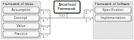
\includegraphics[scale=0.9]{figures/framework}
  \caption{
    The two subframeworks of the Arrowhead framework, concerned with \textit{ideas} and \textit{software}.
    The specifications and implementations of the software framework must conform to the assumptions, concepts, values and practices of the idea framework.
    The concepts of the idea framework are outlined in this document.
  }
  \label{fig:framework}
\end{figure}

This document is part of Arrowhead's framework of ideas.
As such, it is primarily concerned with defining concepts.
However, before we move on to consider our overview those concepts, we will first present a few examples of other key framework ideas.\footnote{
  At the time of writing, the best source of assumptions, values and practices of the Arrowhead framework is Jerker Delsing's book \textit{{IoT} Automation: Arrowhead Framework} \cite{delsing2017iot}.
  The \GlossaryHyperRef{project-eclipse-arrowhead}{Eclipse Arrowhead project} may publish other works of relevance in the future.
}
It is, for example, \textit{assumed} that the framework may be applied in contexts where the primary activity is markedly physical, such as in transportation, mining, manufacturing, electricity generation, healthcare, and so on.
One of the system characteristics \textit{valued} by the framework is \textit{resilience}, or the expectation that every system should do its outmost to mitigate and recover from degradations, failures or other contingencies that may affect its ability to perform its designated tasks.
Finally, one of its \textit{recommended practices} is that every system-of-systems should be thoroughly documented at every level, from its smallest components up to its most high-level interactions.

The rest of this section gives an overview of the most fundamental concepts of the framework.
It is meant to prepare you for the next section, where the same concepts, and other supporting concepts, are presented in greater detail.

\subsection{Stakeholders and Artifacts}

There are two kinds of members of the world of Arrowhead, (1) \GlossaryHyperRef{stakeholder}{stakeholders} and (2) \GlossaryHyperRef{artifact}{artifacts}, as depicted in Figure \ref{fig:world}.
The former denotes a \GlossaryHyperRef{person}{person} or \GlossaryHyperRef{organization}{organization} engaged in an Arrowhead enterprise, while the latter is any thing or object, tangible or intangible, that could be relevant to consider as part of such an enterprise.
Stakeholders \GlossaryHyperRef{owner}{own}, \GlossaryHyperRef{supplier}{supply}, \GlossaryHyperRef{developer}{develop}, \GlossaryHyperRef{operator}{operate}, and \GlossaryHyperRef{user}{use} artifacts, among many other possible activities.
It is their business needs and ambitions that govern what and how Arrowhead artifacts are employed.

\vfill

\begin{figure}[ht!]
  \centering
  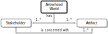
\includegraphics[scale=0.9]{figures/world}
  \caption{
    The two kinds of members of the Arrowhead world: stakeholders and artifacts.
  }
  \label{fig:world}
\end{figure}

\subsection{Devices, Systems and Services}

The most essential types of artifacts in the world of Arrowhead are (1) \GlossaryHyperRef{device}{hardware devices}, (2) \GlossaryHyperRef{system}{software systems} and (3) \GlossaryHyperRef{service}{services}, all shown in Figure \ref{fig:device-system-service}.
\textit{Hardware devices}, or just \textit{devices}, are physical machines, such as servers, robots or tools, that are able to maintain, or \GlossaryHyperRef{hosting-system}{\textit{host}}, \textit{software systems}.
A software system, or just \textit{system}, is a \GlossaryHyperRef{communication}{communicating} \GlossaryHyperRef{instance-software}{software instance} that \GlossaryHyperRef{provision-service}{provides} \textit{services}.
Every service represents a set of tasks a system can perform for other systems or for its stakeholders.
When a system or stakeholder makes use of a service, it is said to \GlossaryHyperRef{consumption-service}{\textit{consume}} it.

\vfill

\begin{figure}[ht!]
  \centering
  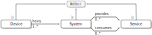
\includegraphics[scale=0.9]{figures/device-system-service}
  \caption{
    Hardware devices \textit{host} software systems, which \textit{consume} and/or \textit{provide} services.
  }
  \label{fig:device-system-service}
\end{figure}

\vfill

Every service represents one area of concern its hosting system can address.
Examples of such areas of concern could be generating financial statements, replacing propellers on drones, manufacturing bolts or measuring humidity.
A service providing control over a door could, for example, make it possible to check if the door is open, to open it and to close it.
Each such activity of every service is represented by one \GlossaryHyperRef{operation-service}{service operation}, which we will consider more in the next section.

\subsection{Service Provision and Consumption}

As we have already established, \GlossaryHyperRef{communication}{communication} between systems is formulated in terms of the \GlossaryHyperRef{provision-service}{provision} and \GlossaryHyperRef{consumption-service}{consumption} of \GlossaryHyperRef{service}{services}.
\GlossaryHyperRef{system}{Systems} may \textit{provide} services, which other systems can \textit{consume} by sending \GlossaryHyperRef{message}{messages} to their \GlossaryHyperRef{operation-service}{operations}, as depicted in Figure \ref{fig:service-consumption}.

\vfill

\begin{figure}[ht!]
  \centering
  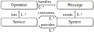
\includegraphics[scale=0.9]{figures/service-consumption}
  \caption{
    Systems consume services by sending messages to the providers of those services.
    Those providers then pass on the messages they receive to their service operations, which interpret and handle them.
  }
  \label{fig:service-consumption}
\end{figure}

\vfill

Also \GlossaryHyperRef{person}{persons} can consume services, even though it is not explicitly depicted in Figure \ref{fig:service-consumption}.
This, however, requires that a \GlossaryHyperRef{interface-human}{human interface} is attached to the providing system, or that another system with such an interface can act as \GlossaryHyperRef{proxy}{proxy}.
The human interface enables the person, via its buttons, prompts or other elements, to send messages to the services in question, just as a regular system would.

When a providing system receives a message from a consuming system or person, it passes it on to the service operation specified in that message, as described in Sections \ref{sec:concepts:service} and \ref{sec:concepts:interface}.
The operation receiving the message will then handle it by performing whatever action it describes, given that the message is \GlossaryHyperRef{message-valid}{valid} and \GlossaryHyperRef{message-permitted}{permitted}.
This handling may entail sending additional messages to other systems, starting or stopping various kinds of automation routines, reading from sensors, electronically signing contracts, sending notifications to an \GlossaryHyperRef{operator}{operator}, sending one or more messages back to the sender, among many other possible examples.

\subsection{System Composition}
\label{sec:overview:system-composition}

\GlossaryHyperRef{system}{Systems} will typically \GlossaryHyperRef{consumer-service}{consume services} because it is a necessary part of executing the tasks they were designed to perform.
Consider, for example, a scenario in which a number of automated guided vehicles, each of which is a system, are to move items around a factory as directed by a scheduling system.
As the scheduling system does not have wheels, engine or other necessary sensors and actuators, it cannot physically move any items by itself. 
Likewise, the individual vehicles are not capable of themselves deciding what needs to be taken to what location.
However, when these different systems cooperate by consuming each others' services, they become able to do things none of them could by themselves.
The combination of scheduling system and vehicles becomes able to plan, track and execute the moving of items.
When systems consume each other's services in this manner, they form a so-called \GlossaryHyperRef{system-of-systems}{system-of-systems}.
Such a system-of-systems is often capable of performing activities none of its constituent \GlossaryHyperRef{subsystem}{subsystems} could perform on its own.

As depicted in Figure \ref{fig:systems-of-systems}, there are different kinds of systems-of-systems with their own characteristics.
There are \GlossaryHyperRef{cloud}{clouds} and \GlossaryHyperRef{system-of-clouds}{systems-of-clouds}, as well as \textit{local} and \textit{virtual} variants of both.

\vfill

\begin{figure}[ht!]
  \centering
  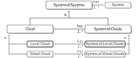
\includegraphics[scale=0.9]{figures/systems-of-systems}
  \caption{
    The different kinds of \textit{systems-of-systems}, each of which consists of a number of \textit{systems} that consume each others' services.
    Clouds are systems-of-systems with \textit{boundaries} and \textit{resource pools}, while systems-of-clouds combine multiple clouds.
  }
  \label{fig:systems-of-systems}
\end{figure}

\vfill

When a system-of-systems has at least one \GlossaryHyperRef{boundary-cloud}{boundary} and at least one pool of \GlossaryHyperRef{resource}{resources}, we refer to it as a \textbf{cloud}.
Boundaries may be formed via access control policies, firewalls, gateway systems, physical separation, among many other possible examples.
Pools of resources may consist of mining equipment, \GlossaryHyperRef{unit-compute}{compute units}, sand, or whatever else is used by the cloud in question to render its services.
Because the Arrowhead framework is highly concerned with physical automation processes, we distinguish \GlossaryHyperRef{cloud-local}{local clouds} from \GlossaryHyperRef{cloud-virtual}{virtual clouds}.

The \textbf{local cloud} has \GlossaryHyperRef{boundary-local}{local boundaries} and \GlossaryHyperRef{resource-local}{local resources}, which means that it must be associated with a physical location.
Examples of local clouds could be smelting stations, drone control towers, assembly lines, power distribution centers, or the components of a satellite.
Whether it be ore, drones, parts, power cables or a complex mesh of all those things, the resources of these example clouds are all markedly \textit{physical}.
Because of their physicality, it matters \textit{where} the clouds are physically located.
Since physical isolation is a form of physical boundary, each of them has both at least one local boundary and at least one local resource.

On the other hand, a \textbf{virtual cloud} has only \GlossaryHyperRef{boundary-virtual}{virtual boundaries} and \GlossaryHyperRef{resource-virtual}{virtual resources}, which means that the values produced by the cloud are not tied to its physical location.
This is the kind of cloud that underpins much of the modern Internet.
A few companies let out virtual compute, storage and network resources, which their clients rent to provision their own virtual clouds and provide their own virtual services.
A virtual cloud could provide services for forecasting, analysis, design, planning, communication, or digital entertainment, among other possible examples.

Individual clouds may be interconnected to former even larger systems-of-systems, which we then refer to as \textbf{systems-of-clouds}.
The individual clouds may be owned and operated by different departments, subdivisions or teams at the same company, or even by different legal entities.
Some of them may be local, while other may be virtual.
Examples of systems-of-clouds may be a set of weather stations operated by the same company, the robots of distinct collaborating companies at a mining site, or the carriers of a supply chain.
When a system-of-clouds contain only local clouds, we refer to it as a \GlossaryHyperRef{system-of-local-clouds}{systems-of-local-clouds}.
Likewise, a system-of-clouds with only virtual clouds constitute a \GlossaryHyperRef{system-of-virtual-clouds}{systems-of-virtual-clouds}.


\section{Concepts}
\label{sec:concepts}
% Copyright (c) 2021 Eclipse Arrowhead Project
%
% This program and the accompanying materials are made available under the
% terms of the Eclipse Public License 2.0 which is available at
% http://www.eclipse.org/legal/epl-2.0.
%
% SPDX-License-Identifier: EPL-2.0

With the major themes of the \GlossaryHyperRef{framework-arrowhead}{Arrowhead framework} now established, we proceed to outline its most significant concepts in detail.
Each subsection of this section \GlossaryHyperRef{description}{describes} one of these concepts, which are as follows:

\vfill

\noindent\begin{tabularx}{\textwidth}{@{} p{0.9cm} p{4.3cm} X @{}}

\ref{sec:concepts:stakeholder} & \textbf{\nameref{sec:concepts:stakeholder}} & A person or \GlossaryHyperRef{organization}{organization} engaged in an \GlossaryHyperRef{entity}{entity} or undertaking. \\
\ref{sec:concepts:entity}      & \textbf{\nameref{sec:concepts:entity}}      & An \GlossaryHyperRef{artifact}{artifact} that can be distinguished from all other artifacts. \\
\ref{sec:concepts:device}      & \textbf{\nameref{sec:concepts:device}}      & A physical \GlossaryHyperRef{entity}{entity} with the \GlossaryHyperRef{capability}{capability} of hosting \GlossaryHyperRef{system}{systems}. \\
\ref{sec:concepts:system}      & \textbf{\nameref{sec:concepts:system}}      & A \GlossaryHyperRef{instance-software}{software instance} able to exercise the \GlossaryHyperRef{capability}{capabilities} of its hosting \GlossaryHyperRef{device}{device}. \\
\ref{sec:concepts:service}     & \textbf{\nameref{sec:concepts:service}}     & A set of \GlossaryHyperRef{operation}{operations} \GlossaryHyperRef{provider-service}{provided} by a \GlossaryHyperRef{system}{system} for other systems to \GlossaryHyperRef{consumer-service}{consume}. \\
\ref{sec:concepts:sos}         & \textbf{\nameref{sec:concepts:sos}}         & A set of \GlossaryHyperRef{system}{systems} that jointly facilitate new \GlossaryHyperRef{capability-system}{capabilities}. \\
\ref{sec:concepts:local-cloud} & \textbf{\nameref{sec:concepts:local-cloud}} & A \GlossaryHyperRef{cloud}{cloud} with a \GlossaryHyperRef{boundary-local}{local boundary} and \GlossaryHyperRef{resource-local}{local resources}.\\
\ref{sec:concepts:solc}        & \textbf{\nameref{sec:concepts:solc}}        & A set of \GlossaryHyperRef{cloud-local}{local clouds} that jointly facilitate new \GlossaryHyperRef{capability-system}{capabilities}.\\
\ref{sec:concepts:network}     & \textbf{\nameref{sec:concepts:network}}     & A set of \GlossaryHyperRef{device}{devices} whose \GlossaryHyperRef{system}{systems} can \GlossaryHyperRef{communication}{communicate}.\\
\ref{sec:concepts:interface}   & \textbf{\nameref{sec:concepts:interface}}   & A \GlossaryHyperRef{boundary}{boundary} that can be crossed by the \GlossaryHyperRef{message}{messages} of certain \GlossaryHyperRef{protocol}{protocols}.\\
\ref{sec:concepts:protocol}    & \textbf{\nameref{sec:concepts:protocol}}    & A \GlossaryHyperRef{description}{description} of how \GlossaryHyperRef{message}{messages} may be sent between \GlossaryHyperRef{entity}{entities}.\\
\ref{sec:concepts:policy}      & \textbf{\nameref{sec:concepts:policy}}      & A set of \GlossaryHyperRef{constraint}{constraints} that must be satisfied for an activity to be permitted.\\

\end{tabularx}

\subsection{Stakeholder}
\label{sec:concepts:stakeholder}

A \GlossaryHyperRef{stakeholder}{stakeholder} is a person or \GlossaryHyperRef{organization}{organization} with \GlossaryHyperRef{stake}{stake} in an \GlossaryHyperRef{entity}{entity} or undertaking with relevance to the \GlossaryHyperRef{framework-arrowhead}{Arrowhead framework}, where \textit{stake} is any form of engagement or commitment.
Stake may be concretely expressed by a stakeholder being associated with one or more \GlossaryHyperRef{role-stakeholder}{\textit{roles}}, as illustrated in Figure \ref{fig:stakeholder}.

\vfill

\begin{figure}[ht!]
  \centering
  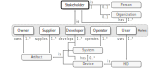
\includegraphics[scale=0.9]{figures/stakeholder}
  \caption{
    The stakeholder as either a person or organization, where each such stakeholder takes on one ore more distinct roles.
    The depicted roles is not an exhaustive list.
    \GlossaryHyperRef{hid}{HID} is an abbreviation for \GlossaryHyperRef{device-human-interface}{Human Interface Device}.
  }
  \label{fig:stakeholder}
\end{figure}

The roles occupied by a given stakeholder dictates what \GlossaryHyperRef{entity}{entities} that person or organization will interact with, as well as the nature of those interaction.
In Figure \ref{fig:stakeholder}, (1) \GlossaryHyperRef{owner}{owner}, (2) \GlossaryHyperRef{supplier}{supplier}, (3) \GlossaryHyperRef{developer}{developer}, (4) \GlossaryHyperRef{operator}{operator} and (5) \GlossaryHyperRef{user}{user} are named explicitly, but more roles are likely to be relevant, such as (6) \GlossaryHyperRef{acquirer}{acquirer} and (7) \GlossaryHyperRef{maintainer}{maintainer}, (8) \GlossaryHyperRef{builder}{builder}, (9) \GlossaryHyperRef{researcher}{researcher} and (10) \GlossaryHyperRef{architect}{architect}.
The listed ten names should be used rather than any synonyms when referring to these particular roles.
Please refer to the \hyperref[sec:glossary]{glossary} for their definitions.
If this document is read electronically, each role name can be clicked to be taken to its definition.

\subsection{Entity}
\label{sec:concepts:entity}

An \GlossaryHyperRef{entity}{entity} is an \GlossaryHyperRef{artifact}{artifact} that can be distinguished from all other artifacts.
We use the word \textit{artifact} to refer to any object or thing, physical or intangible.
As depicted in Figure \ref{fig:entity}, this means that an entity always has an \GlossaryHyperRef{identity}{identity}.

\vfill

\begin{figure}[ht!]
  \centering
  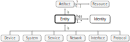
\includegraphics[scale=0.9]{figures/entity}
  \caption{
    The entity as an artifact with an identity.
    An entity or artifact may or may not be considered to be a \GlossaryHyperRef{resource}{resource}, in which case it is deemed to be valuable or useful from the perspective of a \GlossaryHyperRef{stakeholder}{stakeholder}.
    The group of entity types is not exhaustive.
    Other examples are \GlossaryHyperRef{cloud-local}{local clouds}, certain \GlossaryHyperRef{data}{data}, \GlossaryHyperRef{policy}{policies} and \GlossaryHyperRef{profile}{profiles}.
  }
  \label{fig:entity}
\end{figure}


Note that having an identity is not the same as being associated with an \GlossaryHyperRef{identifier}{identifier}, which is a name, number or other value referring to an entity.
It is enough that any such identifier is possible to produce for an artifact to count as an entity.
That being said, certain \GlossaryHyperRef{identification}{identification} requirements, perhaps related to security, performance or discoverability, may make it practically unfeasible not to use identifiers.

\subsection{Device}
\label{sec:concepts:device}

A \GlossaryHyperRef{device}{device} is a physical \GlossaryHyperRef{entity}{entity} with the significant \GlossaryHyperRef{capability}{capability} of being able to host at least one \GlossaryHyperRef{system}{system}, each of which may be given the opportunity to exercise the capabilities of that device.
Examples of capabilities include moving robotic arms, reading from sensors, running \GlossaryHyperRef{procedure-software}{software procedures}, and sending \GlossaryHyperRef{message}{messages}. 
Every device consists of \GlossaryHyperRef{component-hardware}{hardware components}.
While there are no limits to what components can make up a device, each device must always have (1) \GlossaryHyperRef{unit-memory}{memory}, (2) \GlossaryHyperRef{unit-compute}{compute} and (3) \GlossaryHyperRef{interface-device}{interfacing} components, as shown in Figure \ref{fig:device}.

\vfill

\begin{figure}[ht!]
  \centering
  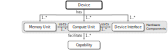
\includegraphics[scale=0.9]{figures/device}
  \caption{
    The device as an entity with hardware components, together facilitating one or more capabilities.
    Devices must be able to host systems, even if not made explicit by this figure.
    Other examples of hardware components part of a device could be sensors, actuators, compute accelerators, or batteries.
  }
  \label{fig:device}
\end{figure}

A device \GlossaryHyperRef{hosting-system}{\textit{hosts}} a system by executing the \GlossaryHyperRef{software}{software} of that system in one or more of its compute units.
Devices must be able to host systems, or they must be considered as hardware components.
While it may seem unintuitive to consider certain machines as components, such as large pumping complexes or vehicles with only manual controls, the \GlossaryHyperRef{framework-arrowhead}{Arrowhead framework} is meant to facilitate automation through the use of interconnected devices with compute capabilities.
If a machine cannot run software, making it able to host systems, that capability must be added before it can play a meaningful role in an \GlossaryHyperRef{arrowhead}{Arrowhead} context.
Consequently, machines without system hosting capabilities must either be considered as components or not be considered from the perspective of Arrowhead at all.

\subsection{System}
\label{sec:concepts:system}

A \GlossaryHyperRef{system}{system} is an \GlossaryHyperRef{identification}{identifiable} \GlossaryHyperRef{instance-software}{software instance} that is able to exercise the \GlossaryHyperRef{capability}{capabilities} of its \GlossaryHyperRef{hosting-system}{hosting} \GlossaryHyperRef{device}{device}.
As shown in Figure \ref{fig:system}, systems consists of \GlossaryHyperRef{component-software}{software components}.
Some significant such components are (1) \GlossaryHyperRef{state-software}{states}, (2) \GlossaryHyperRef{procedure-software}{procedures} and (3) \GlossaryHyperRef{interface-system}{system interfaces}.
A system with these components should be able to \GlossaryHyperRef{consumer-service}{consume} and/or \GlossaryHyperRef{provider-service}{provide} \GlossaryHyperRef{service}{services}, or it must be referred to as an \GlossaryHyperRef{system-isolated}{\textit{isolated system}}.

\begin{figure}[ht!]
  \centering
  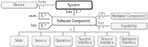
\includegraphics[scale=0.9]{figures/system}
  \caption{
    The system as a collection of related software components, able to facilitate new capabilities.
    While not made explicit by this figure, all software components are \GlossaryHyperRef{hosting-software}{hosted} by either hardware or software components, which means that they use and/or are maintained by those components.
    Examples of software components could be operating systems, file systems, software libraries, programming language runtimes, databases or virtual machines.
  }
  \label{fig:system}
\end{figure}

This rather open-ended definition of ``system'' makes it possible for such to be realized in many ways.
A system may or may not run in its own operating system process, use a certain virtual machine, and so on.

\subsection{Service}
\label{sec:concepts:service}

A \GlossaryHyperRef{service}{service} is an \GlossaryHyperRef{identification}{identifiable} set of \GlossaryHyperRef{operation-service}{operations}, where each operation represents a significant set of activities the \GlossaryHyperRef{system}{system} \GlossaryHyperRef{provider-service}{providing} the service can perform.
Operations are \GlossaryHyperRef{procedure-software}{software procedures} that can be executed by sending \GlossaryHyperRef{message}{messages} to them via their \GlossaryHyperRef{interface-operation}{interfaces}.
The sender of such a message is referred to as a \GlossaryHyperRef{consumer-service}{service consumer}.
As depicted in Figure \ref{fig:service}, an operation may use the \GlossaryHyperRef{capability-system}{capabilities} of its providing system to perform its activities and must ensure certain \GlossaryHyperRef{policy}{policies} are enforced before handling any received messages.

%Other systems may consume such a service by sending a \GlossaryHyperRef{message}{message} via the interface of an operation part of that service.
%If the sent message is \GlossaryHyperRef{message-valid}{valid} and \GlossaryHyperRef{message-permitted}{permitted}, the providing system should use its \GlossaryHyperRef{capability}{capabilities} to perform whatever request is described by that message.

\vfill

\begin{figure}[ht!]
  \centering
  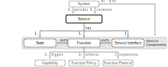
\includegraphics[scale=0.9]{figures/service}
  \caption{
    The service as a set of operations made available via a provider interface, making it possible for a providing system to offer the use of its capabilities to consuming systems.
    Every entity depicted in this figure, except for the \textit{System} and the \textit{Capability}, may be a \GlossaryHyperRef{component-software}{\textit{Software Component}}.
    Each \GlossaryHyperRef{protocol-operation}{\textit{Operation Protocol}} extends $0..1$ \GlossaryHyperRef{protocol-service}{\textit{Service Protocol}}, even if not explicitly denoted in this graph diagram.
  }
  \label{fig:service}
\end{figure}

A \textit{valid} message is such that conforms to the \GlossaryHyperRef{protocol-operation}{protocol} of an operation, while a \textit{permitted} message is such that conforms to all of its \GlossaryHyperRef{policy-operation}{policies}.
Protocols and policies are described further in Sections \ref{sec:concepts:protocol} and \ref{sec:concepts:policy}, respectively.
Operations receive messages via \GlossaryHyperRef{interface-provider}{provider interfaces} and send their own messages via \GlossaryHyperRef{interface-consumer}{consumer interfaces}.
There is no limits on how many messages an invoked operation may send, when they are sent, or who or what is intended to receive them.
When a provider interface receives a message, as described in Section \ref{sec:concepts:interface}, it must \GlossaryHyperRef{routing-message}{route} it to the operation it targets.

\subsection{System-of-Systems}
\label{sec:concepts:sos}

A \GlossaryHyperRef{system-of-systems}{system-of-systems} is a set of at least two \GlossaryHyperRef{system}{systems}, together facilitating one or more \GlossaryHyperRef{capability-system}{capabilities} none of the constituent systems could have on its own.
The facilitation of new capabilities is accomplished by the systems providing services and/or consuming each other's services.

While it may seem as if consuming services would hardly be enough for new capabilities to always emerge, it actually is the case.
For example, let us assume that a system has the capability of turning on and off a light.
That system also provides a service allowing for other systems to request that the light be turned on or off.
If a different system can successfully consume that service, it also gains the capability of turning on and off that particular light.
As a new system now may control that particular light, a new capability has emerged.

\subsection{Local Cloud}
\label{sec:concepts:local-cloud}

A \GlossaryHyperRef{cloud-local}{local cloud} is an \GlossaryHyperRef{identification}{identifiable} \GlossaryHyperRef{system-of-systems}{system-of-systems} able to execute given tasks through the use of a pool of \GlossaryHyperRef{resource}{resources}.
The resource pool of a local cloud could contain 3D-printers, autonomous unmanned vehicles, conventional servers, or anything else producing a value on demand.
As depicted in Figure \ref{fig:local-cloud}, the local cloud is distinct from other types of \GlossaryHyperRef{cloud}{clouds} by having at least one \GlossaryHyperRef{boundary-local}{local boundary} and one \GlossaryHyperRef{resource-local}{local resource}, which means that it is physically tied to a concrete location.
A local cloud could be engaged in manufacturing, repairs, heating, electricity distribution, workspace monitoring, drone fleet control, among many other possible kinds of physical activities.
A local cloud may be stationary or mobile.
A cloud that has no resources or boundaries tied to any particular physical locations should be referred to as a \GlossaryHyperRef{cloud-virtual}{\textit{virtual cloud}}.

\vfill

\begin{figure}[ht!]
  \centering
  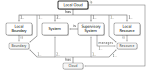
\includegraphics[scale=0.9]{figures/local-cloud}
  \caption{
    The local cloud as a regular cloud with at least one local boundary and one local resource.
  }
  \label{fig:local-cloud}
\end{figure}

That a local cloud has a boundary means that a distinction is being made between \GlossaryHyperRef{system}{systems} inside and outside the cloud.
A boundary being local means that the distinction is being made by a physical \GlossaryHyperRef{attribute}{attribute}, such as device location, type of device, or physical attachment to a certain \GlossaryHyperRef{entity}{entity}.
Boundaries may be protected, which means that measures are in place to guarantee security, safety, real-time characteristics, or other local cloud attributes.
The resources of a local cloud may be of any type, from virtual compute resources to physical drills or pumps.
A system managing a resource may be referred to as a \GlossaryHyperRef{system-supervisory}{\textit{supervisory system}}.

\subsection{System-of-Local-Clouds}
\label{sec:concepts:solc}

A \GlossaryHyperRef{system-of-local-clouds}{system-of-local-clouds} is two or more \GlossaryHyperRef{cloud-local}{local clouds} that \GlossaryHyperRef{consumer-service}{consume} each other's \GlossaryHyperRef{service}{services} to facilitate new \GlossaryHyperRef{capability-system}{capabilities}.
It is similar to the local cloud, with the exception of its \GlossaryHyperRef{subsystem}{subsystems} are \GlossaryHyperRef{cloud-local}{local clouds} instead of plain \GlossaryHyperRef{system}{systems}.
A system-of-local-clouds may have its own \GlossaryHyperRef{boundary-cloud}{boundaries} in addition to those of its constituent local clouds.
Those boundaries are formed by attributes shared by all the constituent local clouds, such as certificates issued by the same organization, or physical attachment to the same network bus.
A system-of-local-clouds cannot have resources beyond those of its constituent clouds, however.

\subsection{Network}
\label{sec:concepts:network}

A \GlossaryHyperRef{network}{network} is an \GlossaryHyperRef{identification}{identifiable} set of two or more \GlossaryHyperRef{device-end}{end devices}, \GlossaryHyperRef{connection}{connected} such that any \GlossaryHyperRef{system}{systems} they host are able to \GlossaryHyperRef{communication}{communicate}.
As shown in Figure \ref{fig:network}, end devices may be \GlossaryHyperRef{interconnection}{interconnected} via \GlossaryHyperRef{device-intermediary}{intermediary devices}.

\vfill

\begin{figure}[ht!]
  \centering
  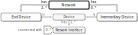
\includegraphics[scale=0.9]{figures/network}
  \caption{
    The network as a set of connected end devices, potentially interconnected by intermediary devices.
  }
  \label{fig:network}
\end{figure}

Both end devices and intermediary devices are regular \GlossaryHyperRef{device}{devices}, which means that they have \GlossaryHyperRef{interface-device}{device interfaces} through which they can send and receive \GlossaryHyperRef{message}{messages}.
Only \GlossaryHyperRef{device-connected}{\textit{connected} devices} can pass messages between their interfaces, however.
Intermediary devices pass on messages toward their intended end devices instead of handling them themselves.
Examples of intermediary devices are routers, switches, and firewalls.
Device interfaces used exclusively for passing on messages are referred to as \GlossaryHyperRef{interface-network}{network interfaces}.
The term ``end device'' should only be used when a distinction needs to be made between end and intermediary devices.

\subsection{Interface}
\label{sec:concepts:interface}

An \GlossaryHyperRef{interface}{interface} is an \GlossaryHyperRef{identification}{identifiable} \GlossaryHyperRef{boundary}{boundary} over which \GlossaryHyperRef{message}{messages} of certain supported \GlossaryHyperRef{protocol}{protocols} may cross.
An interface may pass messages between \GlossaryHyperRef{connection}{connections} and \GlossaryHyperRef{entity}{entities}, between entities, or between entities and \GlossaryHyperRef{person}{persons}.
As outlined in Figure \ref{fig:interface}, there are three types of interfaces of particular relevance in the context of the \GlossaryHyperRef{framework-arrowhead}{Arrowhead framework}, which are (1) \GlossaryHyperRef{interface-device}{device interfaces}, (2) \GlossaryHyperRef{interface-system}{system interfaces}, and (3) \GlossaryHyperRef{interface-service}{service interfaces}.

\vfill

\begin{figure}[ht!]
  \centering
  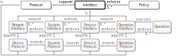
\includegraphics[scale=0.9]{figures/interface}
  \caption{
    The interface as a set of supported protocols and enforced policies.
    Devices, systems, services and operations have their own interface types, each with its corresponding protocol type.
    In the order listed, each interface type may be able to pass on messages to its one or two neighbor types.
  }
  \label{fig:interface}
\end{figure}


%At each level, if a received message satisfies its protocol, it is routed towards its designated recipient.
%If the message does not satisfy its protocol, it is ignored, replied to with an error message, or some other set of actions are performed.
%As depicted in Figure \ref{fig:service}, provider interfaces route messages to \GlossaryHyperRef{operation-service}{service operations}, which may handle them by sending new messages via consumer interfaces.

%Each of these interface levels depend on the layer below it, with the exception of the device interface at the bottom.
%As each interface supports its own set of protocols, each interface layer must support a protocol that extends that of the below layer.
%A device interface may, for example, support the IP \cite{deering2017internet} protocol via Ethernet \cite{iso202188023}, a system interface the HTTP \cite{fielding2014hypertext} protocol via TCP \cite{postel1981transmission}, and a service interface a custom HTTP extension allowing for a target service operation to be specified.
%Note that the protocol at each layer may consist of multiple protocols extending each other, as in this example.
%A particular chain of protocols supported by a device, system or service is referred to as a \GlossaryHyperRef{stack-protocol}{\textit{protocol stack}}.
%The protocol stack of the system in the previous example would be Ethernet, IP, TCP and HTTP, from the bottom and up.

\subsection{Protocol}
\label{sec:concepts:protocol}

A \GlossaryHyperRef{protocol}{protocol} is an \GlossaryHyperRef{identification}{identifiable} \GlossaryHyperRef{description}{description} of how certain \GlossaryHyperRef{message}{messages} may be sent between \GlossaryHyperRef{entity}{entities} as dictated by zero or more \GlossaryHyperRef{state-protocol}{states}.
Received messages may be rejected for violating a current state, or cause a state to be updated.
States may also be updated by temporal events, such as timeouts.
As shown in Figure \ref{fig:protocol}, a protocol may be defined as an \GlossaryHyperRef{protocol-extensible}{extension} of another protocol, as well as be constrained by certain \GlossaryHyperRef{profile-protocol}{profiles} and \GlossaryHyperRef{encoding}{encodings}.

\begin{figure}[ht!]
  \centering
  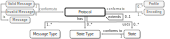
\includegraphics[scale=0.9]{figures/protocol}
  \caption{
    The protocol as set of state and message types, constrained by profiles and encodings.
  }
  \label{fig:protocol}
\end{figure}

Just as a \GlossaryHyperRef{policy}{policy}, a \textit{profile} is a set of constraints.
Unlike the former, however, a profile is limited to only constraining the state types and message types of a protocol.
Profiles can be used to specify how authorization tokens are to be included in messages, or demand that a certain message semantics be observed.
Adding a profile to a protocol not already conforming to it produces a new protocol.

Encodings introduce \GlossaryHyperRef{system-type}{type systems} in which message payloads can be expressed.
If a protocol defines its messages without referring to an encoding, it is considered to have a \textit{custom} encoding.

\subsection{Policy}
\label{sec:concepts:policy}

A \GlossaryHyperRef{policy}{policy} is an \GlossaryHyperRef{identification}{identifiable} set of \GlossaryHyperRef{constraint}{constraints}, useful for determining if given \GlossaryHyperRef{message}{messages} are acceptable or not, as depicted in Figure \ref{fig:policy}.
As messages are always meant to \GlossaryHyperRef{invocation-operation}{invoke operations}

that must be satisfied by a \GlossaryHyperRef{message}{message} for the activity associated with a certain \GlossaryHyperRef{operation-service}{service operation} to be permitted, 
A policy may use any of the \GlossaryHyperRef{capability-system}{capabilities}, or other provisions, of its system to determine if a given message is permitted.
Policies may be concerned with authorization, contracts, economic goals, and so on.
If a \GlossaryHyperRef{message}{message} \GlossaryHyperRef{invocation-operation}{invoking} a particular service operation fails to satisfy one or more of its policies, the sender of that message should be notified about what policies are being violated.

\begin{figure}[ht!]
  \centering
  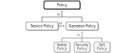
\includegraphics[scale=0.9]{figures/policy}
  \caption{
    The policy as a set of constraints.
    The types of constraints depicted are to be considered only as a limited set of possible examples.
    \GlossaryHyperRef{qos}{QoS} is an abbreviation for \GlossaryHyperRef{service-quality-of}{quality of service}.
  }
  \label{fig:policy}
\end{figure}

While policies are only explicitly associated with operations in this document, a derived work may choose to associate policies also with services, systems, system-of-systems and/or devices.
Such policies must be understood to apply to every operation made available by any such entity.


\section{Conformance Requirements}
\label{sec:conformance}
% Copyright (c) 2021 Eclipse Arrowhead Project
%
% This program and the accompanying materials are made available under the
% terms of the Eclipse Public License 2.0 which is available at
% http://www.eclipse.org/legal/epl-2.0.
%
% SPDX-License-Identifier: EPL-2.0

For a document, \GlossaryHyperRef{model}{model}, or other \GlossaryHyperRef{artifact}{artifact}, to be considered as conformant to the \GlossaryHyperRef{model-reference}{reference model} recorded in this document, the following must be observed by that \textit{derived work}:

\begin{enumerate}
\item At least one of the concepts defined in this reference model must be part of that derived work.
\item The derived work must make it explicit what concepts are taken from this reference model.
	\begin{enumerate}
	\item How this is done most suitably depends on the type of derived work. A document may include a normative reference to this document, while a model may want to give all relevant entities and relations a property with the identity of this document, for example.
	\end{enumerate}
\item Every concept taken from this reference model must be represented by the name it is given here.
	\begin{enumerate}
	\item If important to be able to distinguish an Arrowhead concept from other such of relevance, concepts from this reference model may be qualified by the leading word ``Arrowhead'', as in, for example, ``Arrowhead system`` or ``Arrowhead service function''.
	\item Note that some concepts defined here are given more than one name. For example, \GlossaryHyperRef{function-program}{program function} and \GlossaryHyperRef{procedure-software}{software procedure} are declared to be synonyms in the glossary. When synonyms exist, only one of their entries in the glossary will have a definition. The name of that definition should be the name being used.
	\end{enumerate}
\item Concepts taken from this reference model may be \textit{specialized} or \textit{simplified}, but must never be \textit{contradicted}.
	\begin{enumerate}
	\item \textit{Specialization} means that more \GlossaryHyperRef{constraint}{constraints} are applied to it than are presented here. For example, a certain derived work may require that all devices have \GlossaryHyperRef{unit-compute}{compute units} supporting a certain instruction set, or that every \GlossaryHyperRef{system}{system} \GlossaryHyperRef{provider-service}{provides} a specific monitoring \GlossaryHyperRef{service}{service}, and so on.
	\item \textit{Simplification} means that \GlossaryHyperRef{entity}{entities}, \GlossaryHyperRef{relationship}{relationships} or \GlossaryHyperRef{property}{properties} introduced here are omitted due to being outside the scope of the derived work. For example, a technical document may not be concerned with \GlossaryHyperRef{role-stakeholder}{stakeholder roles}, while a model of certain types of local clouds may not be concerned with whether or not artifacts are \GlossaryHyperRef{resource}{resources} or not, and so on.
	\item \textit{Contradiction} means that a property or other constraint is introduced that makes it impossible to reconcile the concepts presented here with those in the derived work. A derived work must not, for example, demand that no devices ever host systems, or that services be provided directly by devices without them hosting systems, and so on.
	\end{enumerate}
\end{enumerate}

\subsection{ISO/IEC/IEEE 42010}
\label{sec:conformance:iso42010}

\section{Glossary}
\label{sec:glossary}
% Copyright (c) 2021 Eclipse Arrowhead Project
%
% This program and the accompanying materials are made available under the
% terms of the Eclipse Public License 2.0 which is available at
% http://www.eclipse.org/legal/epl-2.0.
%
% SPDX-License-Identifier: EPL-2.0

This section provides an alphabetically sorted list of all significant terms introduced or named in this document.
Each term consisting of more than one word is sorted by its final, or qualified, word.
This means that the definition of \GlossaryHyperRef{protocol-service}{service protocol}, for example, is found at \GlossaryNameRef{protocol-service}.

Many of the definitions are amended with notes and references to RAMI4.0 \cite{adolphs2016reference}, SOA-RM \cite{mackenzie2006reference} and IoTA:AF \cite{delsing2017iot}, which are always listed after the definition they amend.
Regular notes are numbered, while those making a comment on a definition in RAMI4.0, SOA-RM or IoTA:AF are introduced with the three abbreviations just listed.

{

\newcommand{\GlossaryEntry}[3][]{\subsubsection*{#3\IfStrEq{#1}{}{}{ {\normalfont \textit{#1}}}}\label{sec:glossary:#2}}
\newcommand{\GlossaryNote}[2]{\begin{minipage}[b]{\dimexpr\linewidth-0.5cm\relax}\vspace*{0.33cm}\footnotesize{\textbf{#1}\ #2}\end{minipage}}

\GlossaryEntry{abstract}{Abstract}
See \GlossaryNameRef{model-abstract}.

\GlossaryEntry{architecture}{Architecture}
A \GlossaryHyperRef{model-concrete}{concrete model} of a \GlossaryHyperRef{system-of-systems}{system-of-systems} defined in terms of certain \GlossaryHyperRef{model-reference}{reference models}, \GlossaryHyperRef{architecture-reference}{reference architectures} and other concrete architectures.
See Section \ref{sec:introduction:scope}.

	\GlossaryNote{RAMI4.0}{
	    defines architecture as the ``combination of elements of a model based on principles and rules for constructing, refining and using it''.
		We consider ``combinations of elements of a model'' to be a ``model of a system-of-systems'' and to be ``based on principles and rules for constructing, refining and using it'' as building upon reference models and architectures.
		Our definition should be interpreted as being compatible but more specific.
	}

	\GlossaryNote{SOA-RM}{
		defines software architecture as ``the structure or structures of an information system consisting of entities and their externally visible properties, and the relationships among them''.
		That definition is equivalent to our definition of \GlossaryHyperRef{model}{model}, with the exception that the thing being modeled has to be an information system.
		As our definition is concerned with a model and a system-of-systems, which must be an information system, we regard out definition as compatible but more specific.
	}

\GlossaryEntry{architecture-reference}{Architecture, Reference}
A significantly useful \GlossaryHyperRef{model-abstract}{abstract model} of a \GlossaryHyperRef{system-of-systems}{system-of-systems} defined in terms of certain \GlossaryHyperRef{model-reference}{reference models} and other reference architectures.
See Section \ref{sec:introduction:scope}.

	\GlossaryNote{RAMI4.0}{
		defines reference architecture as a ``model for an architecture description (for I[ndustry ]4.0) which is generally used and recognized as being suitable (has reference character)''.
		We consider a ``model for an architecture description'' to be an ``abstract model of a system-of-systems''.
		Our definition should be interpreted as being compatible but more specific.
	}

	\GlossaryNote{SOA-RM}{
	    defines reference architecture as ``an architectural design pattern that indicates how an abstract set of mechanisms and relationships realizes a predetermined set of requirements''.
	    While we let the part about requirements be implicit, our definition should be interpreted as being compatible but more specific.
	}

\GlossaryEntry{architecture-service-oriented}{Architecture, Service-Oriented (SOA)}
An \GlossaryHyperRef{architecture}{architecture} concerned with \GlossaryHyperRef{service}{service} \GlossaryHyperRef{provider-service}{provision} and \GlossaryHyperRef{consumer-service}{consumption}.

	\GlossaryNote{Note 1}{
		Any architecture building upon the \GlossaryHyperRef{model-reference}{reference model} of this document will become service-oriented.
		See also Section \ref{sec:introduction}.
	}

\GlossaryEntry{arrowhead}{Arrowhead}
See \GlossaryNameRef{framework-arrowhead}.

\GlossaryEntry{artifact}{Artifact}
A thing or object, tangible or intangible.

\GlossaryEntry{asset}{Asset}
Synonymous to \GlossaryNameRef{resource}.

	\GlossaryNote{RAMI4.0}{
		defines asset as an ``object which has a value for an organization''.
		See \GlossaryNameRef{resource} for a comparable term.
	}

\GlossaryEntry{attribute}{Attribute}
A name/value pair of \GlossaryHyperRef{data}{data}, associated with either an \GlossaryHyperRef{entity}{entity} or a \GlossaryHyperRef{relationship}{relationship}.

	\GlossaryNote{Note 1}{
		A attribute is a form of \GlossaryHyperRef{metadata}{metadata}.
	}

\GlossaryEntry{boundary}{Boundary}
A point or border where either two or more \GlossaryHyperRef{artifact}{artifacts} meet or one artifact ends.

\GlossaryEntry{boundary-cloud}{Boundary, Cloud}
A \GlossaryHyperRef{boundary}{boundary} separating the \GlossaryHyperRef{artifact}{artifacts} belonging to a \GlossaryHyperRef{cloud}{cloud} from those not belonging to it.

	\GlossaryNote{Note 1}{
		A cloud boundary can be \GlossaryHyperRef{boundary-local}{local} or \GlossaryHyperRef{boundary-virtual}{virtual}, depending on if the boundary is formed by physical or virtual \GlossaryHyperRef{attribute}{attributes}.
	} 

\GlossaryEntry{boundary-local}{Boundary, Local}
A \GlossaryHyperRef{boundary}{boundary} that exists in the physical world.

	\GlossaryNote{Note 1}{
		Local boundaries can be facilitated by walls, locations of operation, attachment to certain vehicles or power sources, and so on.
	}

\GlossaryEntry{boundary-virtual}{Boundary, Virtual}
A \GlossaryHyperRef{boundary}{boundary} that exists only virtually.

	\GlossaryNote{Note 1}{
		Virtual boundaries can be facilitated by cryptographic secrets, identifiers, ownership statements, contracts, and so on.
	}

\GlossaryEntry{capability}{Capability}
A task, of any nature, that can be performed by a \GlossaryHyperRef{device}{device}.

	\GlossaryNote{Note 1}{
		The term must be understood in the most general sense possible.
		It includes the abilities of hosting \GlossaryHyperRef{system}{systems}, reading from sensors, triggering actuators, among many other possible examples.
	}

	\GlossaryNote{SOA-RM}{
		defines a capability as ``a real-world effect that a service provider is able to provide to a service consumer''.
		To leave room for devices to be described as doing other things that \GlossaryHyperRef{provider-service}{providing} or \GlossaryHyperRef{consumer-service}{consuming} services, we made our definition more general.
		See also \GlossaryNameRef{capability-system}.
	}

\GlossaryEntry{capability-system}{Capability, System}
A \GlossaryHyperRef{capability}{capability} a \GlossaryHyperRef{system}{system} can trigger via its hosting \GlossaryHyperRef{device}{device}.

\GlossaryEntry{cloud}{Cloud}
A \GlossaryHyperRef{boundary}{bounded} \GlossaryHyperRef{system-of-systems}{system-of-systems} able independently execute given tasks through the use of a pool of \GlossaryHyperRef{resource}{resources}.

	\GlossaryNote{Note 1}{
		When the term ``cloud'' is used elsewhere, it often refers to clouds with only virtual resources, such as compute, storage and software-defined network utilities.
		Here, we refer to such clouds as \GlossaryHyperRef{cloud-virtual}{virtual clouds}.
		By making the unqualified word ``cloud'' less specific, it becomes more clear how our \GlossaryHyperRef{cloud-local}{local cloud} concept shares similarities with other types of clouds.
	}

\GlossaryEntry{cloud-local}{Cloud, Local}
A \GlossaryHyperRef{cloud}{cloud} \GlossaryHyperRef{boundary-local}{bound to a physical location} due to its acting on or producing \GlossaryHyperRef{resource-local}{local resources}.
See Section \ref{sec:reference-model:system-of-systems:local-cloud}.

	\GlossaryNote{IoTA:AF}{
		provides an introduction to the local cloud concept in its second chapter, as well as an architectural definition in its third chapter.
		The following is an excerpt from the introduction:
		\begin{quote}
		The local cloud concept takes the view that specific geographically local automation tasks should be encapsulated and protected.
		These tasks have strong requirements on real time, ease of engineering, operation and maintenance, and system security and safety.
		The local cloud idea is to let the local cloud include the devices and systems required to perform the desired automation tasks, thus providing a local ``room'' which can be protected from outside activities.
		In other words, the cloud will provide a boundary to the open internet, thus aiming to protect the internal of the local cloud from the open internet.
		\end{quote}
		The third chapter contains the following:
		\begin{quote}
		In the Arrowhead Framework context a local cloud is defined as a self-contained network with the three mandatory core systems deployed and at least one application system deployed [...]
		\end{quote}
		Both of these descriptions are practical, in the sense that they emphasize engineering aspects.
		As this document is a reference model, engineering aspects are out of scope.
		The more general terms ``geographically local'', ``room'' and ``boundary'' clearly highlight the physicality of the local cloud itself, while the depiction of ``devices'' performing ``automation tasks'' makes it apparent that some kind of physical activity is involved, such as manufacturing.
		Finally, the local cloud being ``encapsulated'', ``protected'' and ``self-contained'' indicates that it is understood to exhibit a degree of independence with respect to the tasks it is given, which we expect all kinds of clouds to exhibit.
		Our definition should be interpreted as a summation of these characteristics.
	}

\GlossaryEntry{cloud-local-automation}{Cloud, Local Automation}
See \GlossaryNameRef{cloud-local}.

\GlossaryEntry{cloud-virtual}{Cloud, Virtual}
A \GlossaryHyperRef{cloud}{cloud} \GlossaryHyperRef{boundary-virtual}{unbound by physical location} by only acting on or producing \GlossaryHyperRef{resource-virtual}{virtual resources}.

\GlossaryEntry[(verb)]{code}{Code}
Transforming \GlossaryHyperRef{data}{data} from being expressed in one \GlossaryHyperRef{encoding}{encoding} into another.
See also \GlossaryHyperRef{decode}{decode} and \GlossaryHyperRef{encode}{encode}.

\GlossaryEntry[(noun)]{coding}{Coding}
Synonymous to \GlossaryNameRef{encoding}.

\GlossaryEntry{component}{Component}
An \GlossaryHyperRef{entity}{entity} that can be part of a \GlossaryHyperRef{device}{device} or \GlossaryHyperRef{system}{system} and contribute to it facilitating its \GlossaryHyperRef{capability}{capabilities}.

	\GlossaryNote{Note 1}{
		The word ``component'' should only be used to refer to the constituents of devices and systems.
		It should never be used to refer to a system being a constituent of a \GlossaryHyperRef{system-of-systems}{system-of-systems}.
		Such a system should be referred to as being a \GlossaryHyperRef{subsystem}{subsystem}.
	}

	\GlossaryNote{RAMI4.0}{
		makes no practical distinction between components and systems, as is done here.
		See \GlossaryNameRef{system} for more details.
	}

\GlossaryEntry{component-hardware}{Component, Hardware}
A physical \GlossaryHyperRef{component}{component} that can only be part of a \GlossaryHyperRef{device}{device}.
See Section \ref{sec:reference-model:device}.

\GlossaryEntry{component-software}{Component, Software}
A virtual \GlossaryHyperRef{component}{component} that can only be part of a \GlossaryHyperRef{system}{system}.
See Section \ref{sec:reference-model:system}.

\GlossaryEntry{communication}{Communication}
The activity of sending and/or receiving \GlossaryHyperRef{message}{messages}.

\GlossaryEntry{communication-service-oriented}{Communication, Service-Oriented}
\GlossaryHyperRef{communication}{Communication} \GlossaryHyperRef{description}{described} in terms of the \GlossaryHyperRef{provider-service}{provision} and \GlossaryHyperRef{consumer-service}{consumption} of \GlossaryHyperRef{service}{services}.

\GlossaryEntry{concrete}{Concrete}
See \GlossaryNameRef{model-concrete}.

\GlossaryEntry{concretization}{Concretization}
Making an \GlossaryHyperRef{model-abstract}{abstract model} less abstract by specifying some or all details required to realize it.

\GlossaryEntry{configuration}{Configuration}
A set of changeable \GlossaryHyperRef{attribute}{attributes} that directly influence how a \GlossaryHyperRef{system}{system} exercises its \GlossaryHyperRef{capability-system}{capabilities}.

\GlossaryEntry{configure}{Configure}
To update a \GlossaryHyperRef{configuration}{configuration}.

\GlossaryEntry{connection}{Connection}
An active medium through which attached \GlossaryHyperRef{interface}{interfaces} can \GlossaryHyperRef{communication}{communicate}.

\GlossaryEntry{constraint}{Constraint}
A \GlossaryHyperRef{attribute}{attribute} that imposes constraints, or limits, on an \GlossaryHyperRef{entity}{entity} or \GlossaryHyperRef{relationship}{relationship}.

	\GlossaryNote{Note 1}{
		The presence of constraints enable \GlossaryHyperRef{validation}{validation}.
	}

	\GlossaryNote{Note 2}{
		Perhaps a bit counterintuitively, a constraint \textit{adds} information to its target by reducing the ways in which it could be realized.
	}

\GlossaryEntry{consumer-service}{Consumer, Service}
A \GlossaryHyperRef{system}{system} currently \GlossaryHyperRef{invocation-function}{invoking} a \GlossaryHyperRef{function-service}{function} \GlossaryHyperRef{provider-service}{provided} via a \GlossaryHyperRef{service}{service}.

	\GlossaryNote{Note 1}{
		If used to refer to a \GlossaryHyperRef{stakeholder}{stakeholder}, the term must be interpreted as if that stakeholder consumes services via systems.
	}

	\GlossaryNote{SOA-RM}{
		defines a service consumer as ``an entity which seeks to satisfy a particular need through the use [of] capabilities offered by means of a service''.
		We require that the one consuming the service is (1) a \GlossaryHyperRef{system}{system} rather than just any \GlossaryHyperRef{entity}{entity}, as well as (2) that the \GlossaryHyperRef{capability-system}{capabilities} of the consumed service be exercised by invoking a function.
	}

\GlossaryEntry{data}{Data}
A sequence of \GlossaryHyperRef{datum}{datums} recording a set of \GlossaryHyperRef{description}{descriptions} via the structure superimposed by a \GlossaryHyperRef{type-data}{data type}.

	\GlossaryNote{Note 1}{
		Let us assume that some data is going to be sent to a drilling machine.
		The type associated with the data requires that it always consists of 8 bits, organized such that the first 4 bits indicate the speed of drilling in multiples of 100 rotations per minute, while the latter 4 determine how much to lower the drill in multiples of 5 millimeters.
		A \GlossaryHyperRef{state}{state} that could be expressed with those 8 bits is \texttt{0100 1101}.
		If each of the two sequences of 4 bits is treated as a big-endian integer with base 2, they record $4$ and $13$ in decimal notation.
		This would indicate that the drill should spin at $4 * 100 = 400$ rotations per minute and be lowered $13 * 5 = 65$ millimeters.
	}

	\GlossaryNote{Note 2}{
		Without knowledge of the types and context associated with some data, that data cannot be interpreted.
	}

\GlossaryEntry{datum}{Datum}
A variable expressing one out of a set of possible values.
See also \GlossaryNameRef{state}.

	\GlossaryNote{Note 1}{
		A familiar example of a datum may be the bit, or binary digit.
		Its possible set of symbols is $\{0, 1\}$.
	}

\GlossaryEntry{decode}{Decode}
The act of transforming \GlossaryHyperRef{data}{data} from being expressed in a \GlossaryHyperRef{encoding}{encoding} suitable for transmission or storage to another encoding suitable for interpretation.

	\GlossaryNote{Note 1}{
		Decoding is the reverse of \GlossaryHyperRef{encode}{encoding}.
	}

	\GlossaryNote{Note 2}{
		The term can also be used to express the act of a human interpreting data.
	}

\GlossaryEntry{description}{Description}
Facts about an \GlossaryHyperRef{entity}{entity} or \GlossaryHyperRef{entity-class-of}{class of entities}, expressed in the form of a \GlossaryHyperRef{model}{model}, a text, or both.

\GlossaryEntry[(noun)]{design}{Design}
Every document, \GlossaryHyperRef{model}{model} and other record \GlossaryHyperRef{description}{describing} how a certain \GlossaryHyperRef{artifact}{artifact} can be \GlossaryHyperRef{implementation}{implemented}.

\GlossaryEntry[(verb)]{design-verb}{Design}
The activity of producing \GlossaryHyperRef{design}{designs}.

\GlossaryEntry{designer}{Designer}
A \GlossaryHyperRef{stakeholder}{stakeholder} involved in the \GlossaryHyperRef{design-verb}{design} of \GlossaryHyperRef{artifact}{artifacts}.
See Section \ref{sec:reference-model:stakeholder}.

\GlossaryEntry{developer}{Developer}
A \GlossaryHyperRef{stakeholder}{stakeholder} developing the \GlossaryHyperRef{component}{components} that make up \GlossaryHyperRef{device}{devices} and/or \GlossaryHyperRef{system}{systems}.
See Section \ref{sec:reference-model:stakeholder}.

\GlossaryEntry{device}{Device}
A physical \GlossaryHyperRef{entity}{entity} made from \GlossaryHyperRef{component-hardware}{hardware components} with the significant \GlossaryHyperRef{capability}{capability} of being able to host \GlossaryHyperRef{system}{systems}.
See Section \ref{sec:reference-model:device}.

	\GlossaryNote{IoTA:AF}{
		defines device as ``a piece of equipment, machine, hardware, etc. with computational, memory and communication capabilities which hosts one or several Arrowhead Framework systems and can be bootstrapped in an Arrowhead local cloud''.
		The definition provided here should be interpreted as being equivalent.
	}

\GlossaryEntry{device-connected}{Device, Connected}
A \GlossaryHyperRef{device}{device} that is physically attached to at least one other device via their \GlossaryHyperRef{interface-device}{interfaces}, enabling them to \GlossaryHyperRef{communication}{communicate}.

\GlossaryEntry{device-end}{Device, End}
A \GlossaryHyperRef{device-connected}{connected device} being the intended recipient of a \GlossaryHyperRef{message}{message}.

\GlossaryEntry{device-human-interface}{Device, Human Interface (HID)}
A \GlossaryHyperRef{device}{device} that provides sensors and actuators that together make up an \GlossaryHyperRef{interface}{interface} through which a human can exchange messages with one or more \GlossaryHyperRef{system}{systems}.

\GlossaryEntry{device-intermediary}{Device, Intermediary}
A \GlossaryHyperRef{device-connected}{connected device} that receives and forwards \GlossaryHyperRef{message}{messages} toward \GlossaryHyperRef{device-end}{end devices}.

\GlossaryEntry{encode}{Encode}
The act of transforming \GlossaryHyperRef{data}{data} from being expressed in a \GlossaryHyperRef{encoding}{encoding} suitable for interpretation to another encoding suitable for transmission or storage.

	\GlossaryNote{Note 1}{
		Encoding is the reverse of \GlossaryHyperRef{decode}{decoding}.
	}

	\GlossaryNote{Note 2}{
		The term can also be used to express the act of a human recording data.
	}

\GlossaryEntry[(noun)]{encoding}{Encoding}
A \GlossaryHyperRef{model-concrete}{concrete} \GlossaryHyperRef{type-data}{data type} used to structure \GlossaryHyperRef{data}{data} for transmission, storage and/or interpretation.

\GlossaryEntry{engineer-standardization}{Engineer, Standardization}
A \GlossaryHyperRef{stakeholder}{stakeholder} involved in producing and ensuring conformance to standards and other significant specifications.
See Section \ref{sec:reference-model:stakeholder}.

\GlossaryEntry{entity}{Entity}
An \GlossaryHyperRef{artifact}{artifact} with an \GlossaryHyperRef{identity}{identity}, allowing for it to be distinguished from all other artifacts.
See Section \ref{sec:reference-model:entity}.

	\GlossaryNote{Note 1}{
		An entity being uniquely identifiable does not necessarily mean that it is associated with a certificate or \GlossaryHyperRef{identifier}{identifier}.
		It only means that a \GlossaryHyperRef{description}{description} can be rendered that unambiguously refers to the entity in question.
	}

	\GlossaryNote{RAMI4.0}{
		defines entity as an ``uniquely identifiable object which is administered in the information world due to its importance''.
		Our definition should be interpreted as being equivalent.
	}

	\GlossaryNote{SOA-RM}{
	    mentions the word ``entity'' nine times, but provides no explicit definition.
	    We assume their definition to match that of a regular English dictionary, such as ``something that has separate and distinct existence and objective or conceptual reality'' \cite{webster2021entity}.
		Our definition should be interpreted as being equivalent.
	}

\GlossaryEntry{entity-class-of}{Entity, Class of}
A set of \GlossaryHyperRef{entity}{entities} that share a common \GlossaryHyperRef{attribute}{attribute}.

\GlossaryEntry{framework}{Framework}
A set of assumptions, concepts, values and practices that frame a certain problem domain.

	\GlossaryNote{SOA-RM}{
		defines framework as ``a set of assumptions, concepts, values, and practices that constitutes a way of viewing the current environment''.
		Our definition should be interpreted as being equivalent.
	}

\GlossaryEntry{framework-arrowhead}{Framework, Arrowhead}
Either of the \GlossaryHyperRef{framework}{framework of ideas} and the \GlossaryHyperRef{framework-software}{framework of software} maintained by the Arrowhead project.
See Section \ref{sec:arrowhead}.

\GlossaryEntry{framework-software}{Framework, Software}
A set of software specifications, \GlossaryHyperRef{implementation-software}{implementations} and other \GlossaryHyperRef{artifact}{artifacts} meant to help address the problem domain of a certain \GlossaryHyperRef{framework}{framework}.

\GlossaryEntry{function}{Function}
Typically synonymous to \GlossaryNameRef{function-service}.
See Section \ref{sec:reference-model:service}.

	\GlossaryNote{Note 1}{
		The term may be used to refer to both \GlossaryHyperRef{function-program}{program} and \GlossaryHyperRef{function-service}{service} functions, if the context makes it clear that both kinds of functions are relevant.
	}

\GlossaryEntry{function-program}{Function, Program}
Synonymous to \GlossaryNameRef{procedure-software}.

\GlossaryEntry{function-service}{Function, Service}
A \GlossaryHyperRef{procedure-software}{software procedure} that handles \GlossaryHyperRef{message}{messages} it receives from a \GlossaryHyperRef{interface-service}{service interface}.
See Section \ref{sec:reference-model:service}.

\GlossaryEntry{hid}{HID}
See \GlossaryNameRef{device-human-interface}.

\GlossaryEntry{industry40}{Industry 4.0}
The fourth industrial paradigm, primarily characterized by high degrees of computerization, digitization and interconnectivity.
See also \cite{adolphs2016reference}.

\GlossaryEntry{identification}{Identification}
The process through which an \GlossaryHyperRef{entity}{entity} verifies the \GlossaryHyperRef{identity}{identity} of another entity. 

\GlossaryEntry{identifier}{Identifier}
\GlossaryHyperRef{data}{Data} associated with an \GlossaryHyperRef{entity}{entity} that allows for it to be \GlossaryHyperRef{identification}{identified}.

\GlossaryEntry{identity}{Identity}
The aspect or aspects, such as \GlossaryHyperRef{identifier}{identifiers}, that makes an \GlossaryHyperRef{entity}{entity} distinct from all other entities.

\GlossaryEntry{implementation}{Implementation}
The realization of a \GlossaryHyperRef{design}{design} as a set of \GlossaryHyperRef{artifact}{artifacts}.

\GlossaryEntry{implementation-software}{Implementation, Software}
An \GlossaryHyperRef{implementation}{implementation} comprised of executable \GlossaryHyperRef{software}{software} \GlossaryHyperRef{artifact}{artifacts}.

\GlossaryEntry{instance-software}{Instance, Software}
A \GlossaryHyperRef{software}{software artifact} currently being executed by a \GlossaryHyperRef{unit-compute}{compute unit}.

\GlossaryEntry{integrator}{Integrator}
A \GlossaryHyperRef{stakeholder}{stakeholder} tasked with making \GlossaryHyperRef{system}{systems} work together by installing and \GlossaryHyperRef{configure}{configuring} them.
See Section \ref{sec:reference-model:stakeholder}.

\GlossaryEntry{interconnection}{Interconnection}
A \GlossaryHyperRef{connection}{connection} that passes through one or more \GlossaryHyperRef{device-intermediary}{intermediary devices}.

\GlossaryEntry{interface}{Interface}
A \GlossaryHyperRef{boundary}{boundary} where \GlossaryHyperRef{message}{messages} of certain \GlossaryHyperRef{protocol}{protocols} can pass between a \GlossaryHyperRef{connection}{connection} and an \GlossaryHyperRef{entity}{entity}, between two entities, or between an entity and a person.
See Section \ref{sec:reference-model:interface}.

\GlossaryEntry{interface-device}{Interface, Device}
An \GlossaryHyperRef{interface}{interface} through which a \GlossaryHyperRef{device}{device} may send and/or receive \GlossaryHyperRef{message}{messages} to/from a \GlossaryHyperRef{connection}{connection}.

\GlossaryEntry{interface-human}{Interface, Human}
An \GlossaryHyperRef{interface}{interface} through which a person may send and/or receive \GlossaryHyperRef{message}{messages} to/from an \GlossaryHyperRef{entity}{entity}.

\GlossaryEntry{interface-network}{interface, Network}
An \GlossaryHyperRef{interface}{interface} of an \GlossaryHyperRef{device-intermediary}{intermediary device}, primarily intended to be used for passing on \GlossaryHyperRef{message}{messages} toward their intended \GlossaryHyperRef{device-end}{end devices}.

\GlossaryEntry{interface-service}{Interface, Service}
An \GlossaryHyperRef{interface}{interface} through which a certain \GlossaryHyperRef{service}{service} can be \GlossaryHyperRef{consumer-service}{consumed}.

	\GlossaryNote{Note 1}{
		Consuming a service requires that \GlossaryHyperRef{message}{messages} be passed from its \GlossaryHyperRef{device}{device} to its \GlossaryHyperRef{system}{system}, and then from its system to the service itself.
		As the \GlossaryHyperRef{software}{software} making up the service is owned by the system, it is the system that is understood to produce any responses.
		Those are passed on via its device.
	}

	\GlossaryNote{SOA-RM}{
		defines service interface as ``the means by which the underlying capabilities of a service are accessed''.
		Our definition should be interpreted as being equivalent.
	}

\GlossaryEntry{interface-system}{Interface, System}
An \GlossaryHyperRef{interface}{interface} through which a \GlossaryHyperRef{system}{system} may send and/or receive \GlossaryHyperRef{message}{messages} to/from its hosting \GlossaryHyperRef{device}{device}.

	\GlossaryNote{Note 1}{
		The device may either send or respond to messages by its own accord, or pass on messages it receives to and/or from any of its \GlossaryHyperRef{interface-device}{device interfaces}.
	}

\GlossaryEntry{invocation-function}{Invocation, Function}
The attempt to exercise the \GlossaryHyperRef{capability-system}{capabilities} of a \GlossaryHyperRef{system}{system} by sending a \GlossaryHyperRef{message}{message} to one of its \GlossaryHyperRef{function}{functions}.

\GlossaryEntry{manager}{Manager}
A \GlossaryHyperRef{stakeholder}{stakeholder} with strategic, operational or other key responsibility over other \GlossaryHyperRef{stakeholder}{stakeholders} and/or significant \GlossaryHyperRef{entity}{entities}.
See Section \ref{sec:reference-model:stakeholder}.

\GlossaryEntry[(noun)]{message}{Message}
\GlossaryHyperRef{data}{Data} sent or received via an \GlossaryHyperRef{interface}{interface}.

	\GlossaryNote{Note 1}{
		In the context of Arrowhead, messages are primarily sent to \GlossaryHyperRef{invocation-function}{invoke} the \GlossaryHyperRef{function}{functions} of \GlossaryHyperRef{service}{services} \GlossaryHyperRef{provider-service}{provided} by \GlossaryHyperRef{system}{systems}.
		However, sending a message to a function requires it to pass through \GlossaryHyperRef{connection}{connections} and various types of interfaces first, which means that it may be relevant to consider these other entities in relation to messages.
	}

\GlossaryEntry{metadata}{Metadata}
\GlossaryHyperRef{data}{Data} \GlossaryHyperRef{description}{describing} other data.

\GlossaryEntry{model}{Model}
A representation of facts in the form of a graph, consisting of \GlossaryHyperRef{entity}{entities}, \GlossaryHyperRef{relationship}{relationships} and \GlossaryHyperRef{attribute}{attributes}.

	\GlossaryNote{Note 1}{
		Models can be expressed or recorded in many ways, including as visual diagrams, spoken words, text and binary data.
	}

	\GlossaryNote{Note 2}{
		Models can be human-readable, machine-readable, or both.
	}

\GlossaryEntry{model-abstract}{Model, Abstract}
A \GlossaryHyperRef{model}{model} that is \textit{insufficiently} specified to be possible to realize as the \GlossaryHyperRef{artifact}{artifact} it represents.

	\GlossaryNote{Note 1}{
		Abstract models can be referred to by other models, serving as a form of \GlossaryHyperRef{constraint}{constraint}.
		They are commonly used to enforce a degree of uniformity across multiple other models.
	}

\GlossaryEntry{model-concrete}{Model, Concrete}
A \GlossaryHyperRef{model}{model} that is \textit{sufficiently} specified to be possible to realize as the \GlossaryHyperRef{artifact}{artifact} it represents.

	\GlossaryNote{Note 1}{
		Two examples of artifacts that could be produced from a concrete model are concrete \GlossaryHyperRef{protocol}{protocols}, the \GlossaryHyperRef{message}{messages} of which can be practically \GlossaryHyperRef{code}{coded}, and \GlossaryHyperRef{implementation-software}{software implementations}.
	}

\GlossaryEntry{model-information}{Model, Information}
A \GlossaryHyperRef{model}{model} consisting of related \GlossaryHyperRef{type-data}{data types}, \GlossaryHyperRef{message}{messages} and/or other information \GlossaryHyperRef{artifact}{artifacts}.

	\GlossaryNote{Note 1}{
		For example, all data types used by a certain \GlossaryHyperRef{service}{service} make up the information model of that service.
		In other words, the concept represents a pool of information artifacts that can are useful to consider as belonging to the same group.
	}

\GlossaryEntry{model-reference}{Model, Reference}
An \GlossaryHyperRef{model-abstract}{abstract model} defining technical concepts of fundamental importance to a specific problem domain.
See also Section \ref{sec:introduction:scope}.

	\GlossaryNote{RAMI4.0}{
		defines reference model as a ``model that is generally used and recognized as being suitable (has recommendation character) for deriving specific models''.
		We understand their use of the word ``specific'' to be equivalent to how we use ``concrete''.
		Even though our definition clarifies that the model in question must be abstract, it should be interpreted as being equivalent.
	}

	\GlossaryNote{SOA-RM}{
		defines reference model as ``an abstract framework for understanding significant relationships among the entities of some environment that enables the development of specific architectures using consistent standards or specifications supporting that environment''.
		It further clarifies that a ``reference model consists of a minimal set of unifying concepts, axioms and relationships within a particular problem domain, and is independent of specific standards, technologies, implementations, or other concrete details''.
		Our definition should be interpreted as being equivalent.
	}

\GlossaryEntry{network}{Network}
A set of two or more \GlossaryHyperRef{device-end}{end devices}, \GlossaryHyperRef{connection}{connected} in such a manner that any \GlossaryHyperRef{system}{systems} they host are able to \GlossaryHyperRef{communication}{communicate}.
See Section \ref{sec:reference-model:network}.

\GlossaryEntry{operator}{Operator}
A \GlossaryHyperRef{stakeholder}{stakeholder} responsible for the \GlossaryHyperRef{configure}{configuration} and oversight of \GlossaryHyperRef{system}{systems} and the \GlossaryHyperRef{resource}{resources} those systems manage.
See Section \ref{sec:reference-model:stakeholder}.

\GlossaryEntry{owner}{Owner}
A \GlossaryHyperRef{stakeholder}{stakeholder} that owns significant \GlossaryHyperRef{resource}{resources} and/or other \GlossaryHyperRef{artifact}{artifacts}.
See Section \ref{sec:reference-model:stakeholder}.

\GlossaryEntry{organization}{Organization}
A \GlossaryHyperRef{stakeholder}{stakeholder} comprised of an organized body of other stakeholders and/or other persons.

\GlossaryEntry{policy}{Policy}
A set of \GlossaryHyperRef{constraint}{constraints}, of any nature, that must be satisfied for a certain activity to be permitted.
See Section \ref{sec:reference-model:policy}.

	\GlossaryNote{SOA-RM}{
		defines policy as ``a statement of obligations, constraints or other conditions of use of an owned entity as defined by a participant''.
		Our definition should be interpreted as being equivalent.
	}

\GlossaryEntry{policy-function}{Policy, Function}
A \GlossaryHyperRef{policy}{policy} that must be satisfied to be permitted to \GlossaryHyperRef{invocation-function}{invoke} a certain \GlossaryHyperRef{function}{function}.

\GlossaryEntry{policy-service}{Policy, Service}
A \GlossaryHyperRef{policy}{policy} that must be satisfied to be permitted to \GlossaryHyperRef{invocation-function}{invoke} any \GlossaryHyperRef{function-service}{function} part of a certain \GlossaryHyperRef{service}{service}.

\GlossaryEntry{procedure}{Procedure}
See \GlossaryNameRef{procedure-software}.

\GlossaryEntry{procedure-software}{Procedure, Software}
A segment of instructions, part of a \GlossaryHyperRef{software}{software artifact}, that perform some activity if executed.

\GlossaryEntry{profile}{Profile}
See \GlossaryNameRef{profile-protocol}.

\GlossaryEntry{profile-protocol}{Profile, Protocol}
A set of \GlossaryHyperRef{constraint}{constraints} superimposed on a \GlossaryHyperRef{protocol}{protocol}.

	\GlossaryNote{Note 1}{
		A profile \textit{never} introduces more \GlossaryHyperRef{message}{messages} to a protocol.
		It adds constraints to the existing messages of a protocol.
	}

	\GlossaryNote{Note 2}{
		A profile could, for example, introduce an authentication mechanism to a protocol by requiring that a certain type of token be included in each message.
		It could demand that a certain protocol be extended, or that a particular kind of \GlossaryHyperRef{encoding}{encoding} be used for message bodies, and so on.
	}

\GlossaryEntry{protocol}{Protocol}
A \GlossaryHyperRef{model}{model} of communication defined in terms of \GlossaryHyperRef{state}{states} and \GlossaryHyperRef{message}{messages}.
See Section \ref{sec:reference-model:protocol}.

	\GlossaryNote{Note 1}{
		The states, if any, dictate the outcomes of sending certain messages.
		For example, let us assume that some state can be either \texttt{BUSY} or \texttt{READY}.
		If the former state would be the active when a certain message is received, the designated response could be an error message.
		If, however, the \texttt{READY} state would have been active, the state could be transitioned to the \texttt{BUSY} value and a success response be provided to the sender.
	}

\GlossaryEntry{protocol-device}{Protocol, Device}
A \GlossaryHyperRef{protocol}{protocol} implemented by a \GlossaryHyperRef{device}{device}.

\GlossaryEntry{protocol-extensible}{Protocol, Extensible}
A \GlossaryHyperRef{protocol}{protocol} allowing for \GlossaryHyperRef{subprotocol}{subprotocols} to be formulated in terms of its \GlossaryHyperRef{message}{messages}.
See also \GlossaryNameRef{stack-protocol}.

	\GlossaryNote{Note 1}{
		Every new message introduced by a subprotocol must be a \GlossaryHyperRef{validation}{valid} message of its \GlossaryHyperRef{superprotocol}{superprotocol}.
	}

	\GlossaryNote{Note 2}{
		Many of the currently prevalent protocols are designed with the intent of being extensible.
		For example, HTTP \cite{fielding2014hypertext} provides provisions for an extending protocol to define its own set of directory operations, to simultaneously support multiple \GlossaryHyperRef{encoding}{codecs}, and so on.
	}

	\GlossaryNote{Note 3}{
		As long as a given protocol provides at least one message whose contents can be arbitrary, a subprotocol can be produced.
		This means that even protocols not designed to be extended can, in some context, be meaningfully used to define subprotocols.
	}

\GlossaryEntry{protocol-function}{Protocol, Function}
A \GlossaryHyperRef{protocol}{protocol} implemented by a \GlossaryHyperRef{function-service}{service function}.

	\GlossaryNote{Note 1}{
		A function protocol is always an \GlossaryHyperRef{protocol-extensible}{extension} of a \GlossaryHyperRef{protocol-service}{service protocol}.
		See Section \ref{sec:reference-model:protocol} for more details.
	}

\GlossaryEntry{protocol-service}{Protocol, Service}
A \GlossaryHyperRef{protocol}{protocol} implemented by a \GlossaryHyperRef{service}{service}.

	\GlossaryNote{Note 1}{
		A service protocol is always an \GlossaryHyperRef{protocol-extensible}{extension} of a \GlossaryHyperRef{protocol-system}{system protocol}.
		See Section \ref{sec:reference-model:protocol} for more details.
	}

\GlossaryEntry{protocol-system}{Protocol, System}
A \GlossaryHyperRef{protocol}{protocol} implemented by a \GlossaryHyperRef{system}{system}.

	\GlossaryNote{Note 1}{
		A system protocol is always an \GlossaryHyperRef{protocol-extensible}{extension} of a \GlossaryHyperRef{protocol-device}{device protocol}.
		See Section \ref{sec:reference-model:protocol} for more details.
	}

\GlossaryEntry{provider-service}{Provider, Service}
A \GlossaryHyperRef{system}{system} that makes \GlossaryHyperRef{service}{services} available for \GlossaryHyperRef{consumer-service}{consumption} to other systems.

	\GlossaryNote{Note 1}{
		If used to refer to a \GlossaryHyperRef{stakeholder}{stakeholder}, the term must be interpreted as if that stakeholder provides services via systems.
	}

	\GlossaryNote{SOA-RM}{
		defines a service provider as ``an entity (person or organization) that offers the use of capabilities by means of a service''.
		Our definition is more specific in that it requires the \GlossaryHyperRef{entity}{entity} be a system.
	}

\GlossaryEntry{qos}{QoS}
See \GlossaryNameRef{service-quality-of}.

\GlossaryEntry{relationship}{Relationship}
A uni-directional association of two \GlossaryHyperRef{entity}{entities}, possibly with an associated \GlossaryHyperRef{data}{data} name.

\GlossaryEntry{researcher}{Researcher}
A \GlossaryHyperRef{stakeholder}{stakeholder} involved in the analysis or development of significant \GlossaryHyperRef{entity}{entities}, particularly with the ambition of facilitating \GlossaryHyperRef{attribute}{attributes} or use cases that cannot be realized without refining, extending or replacing those entities.
See Section \ref{sec:reference-model:stakeholder}.

\GlossaryEntry{resource}{Resource}
An \GlossaryHyperRef{artifact}{artifact} that is of value to a \GlossaryHyperRef{stakeholder}{stakeholder}.

	\GlossaryNote{Note 1}{
		Any type of artifact can be a resource, which includes everything from \GlossaryHyperRef{resource-local}{local resources}, such as raw materials on \GlossaryHyperRef{device}{devices}, to \GlossaryHyperRef{resource-virtual}{virtual resources}, such as \GlossaryHyperRef{system}{systems} or \GlossaryHyperRef{data}{data}.
	}

	\GlossaryNote{Note 2}{
		An artifact stops be a resource when it is perceived as having no value, at which point it may be destroyed, recycled or sold to someone that does perceive it as a resource, for example.
	}

\GlossaryEntry{resource-local}{Resource, Local}
A \GlossaryHyperRef{resource}{resource} whose value is inextricably tied to a physical \GlossaryHyperRef{attribute}{attribute}.

	\GlossaryNote{Note 1}{
		Examples of local resources could be raw materials, drills, pumps, power stations, or drones.
	}

\GlossaryEntry{resource-virtual}{Resource, Virtual}
A \GlossaryHyperRef{resource}{resource} whose value is not derived from any physical \GlossaryHyperRef{attribute}{attribute}.

	\GlossaryNote{Note 1}{
		Examples of virtual resources could be compute, storage, or software-defined network utilities.
	}

\GlossaryEntry{role}{Role}
See \GlossaryNameRef{role-stakeholder}.

\GlossaryEntry{role-stakeholder}{Role, Stakeholder}
An assignment, objective, or other responsibility, that makes a person or organization into a \GlossaryHyperRef{stakeholder}{stakeholder}. 

\GlossaryEntry{router}{Router}
See \GlossaryNameRef{router-message}.

\GlossaryEntry{router-message}{Router, Message}
A \GlossaryHyperRef{component-hardware}{hardware component} or \GlossaryHyperRef{procedure-software}{software procedure} that receives and passes on \GlossaryHyperRef{message}{messages} toward their intended end \GlossaryHyperRef{entity}{entities}.

\GlossaryEntry{routing-message}{Routing, Message}
The act of forwarding a \GlossaryHyperRef{message}{message} towards the \GlossaryHyperRef{function}{function} it is meant to \GlossaryHyperRef{invocation-function}{invoke}.

\GlossaryEntry{service}{Service}
A set of \GlossaryHyperRef{function-service}{functions} that can be \GlossaryHyperRef{provider-service}{provided} by a \GlossaryHyperRef{system}{system} via one or more \GlossaryHyperRef{interface-service}{service interfaces}.
See Section \ref{sec:reference-model:service}.

	\GlossaryNote{RAMI4.0}{
		defines a service as ``separate scope of functions offered by an entity or organization via interfaces''.
		Our definition restricts service provision to systems.
	}

	\GlossaryNote{SOA-RM}{
		defines a service as ``the means by which the needs of a consumer are brought together with the capabilities of a provider''.
		Our definition is more specific about how the \GlossaryHyperRef{capability-system}{capabilities} of a service are made available.
	}

	\GlossaryNote{IoTA:AF}{
		defines a service as ``what [is] used to exchange information from a providing system to a consuming system''.
		It further adds that ``in a service, capabilities are grouped together if they share the same context''.
		The definition presented here should be interpreted as being compatible but more specific about how information is exchanged and capabilities are \GlossaryHyperRef{invocation-function}{invoked}.
	}

\GlossaryEntry{service-quality-of}{Service, Quality of (QoS)}
The degree of performance at which a given \GlossaryHyperRef{service}{service} is \GlossaryHyperRef{provider-service}{provided}. 

\GlossaryEntry{soa}{SOA}
See \GlossaryNameRef{architecture-service-oriented}.

\GlossaryEntry{software}{Software}
A set of sequences of instructions that can be executed by a \GlossaryHyperRef{unit-compute}{compute unit}.

\GlossaryEntry{solc}{SoLC}
See \GlossaryNameRef{system-of-local-clouds}.

\GlossaryEntry{sos}{SoS}
See \GlossaryNameRef{system-of-systems}.

\GlossaryEntry{stack-extensible-protocol}{Stack, Extensible Protocol}
A \GlossaryHyperRef{stack-protocol}{protocol stack} whose topmost \GlossaryHyperRef{protocol}{protocol} is \GlossaryHyperRef{protocol-extensible}{extensible}.

\GlossaryEntry{stack-protocol}{Stack, Protocol}
A stack with an \GlossaryHyperRef{protocol-extensible}{extensible protocol} as base and $n > 0$ \GlossaryHyperRef{subprotocol}{subprotocols} layered on top of it.

	\GlossaryNote{Note 1}{
		Every protocol part of a protocol stack, with the exception of the topmost, must be extensible.
	}

	\GlossaryNote{Note 2}{
		An example of a notable protocol stack is that of HTTP \cite{fielding2014hypertext}.
		It is defined as an extension of the TCP protocol, which in turn extends the IP protocol, which can work as a subprotocol of several other lower-level protocols.
		HTTP is an \GlossaryHyperRef{stack-extensible-protocol}{extensible protocol stack}, which allows for an engineer to define an application-specific protocol on top of its stack.
	}

\GlossaryEntry{stake}{Stake}
Any type of engagement or commitment.

\GlossaryEntry{stakeholder}{Stakeholder}
A person or \GlossaryHyperRef{organization}{organization} with \GlossaryHyperRef{stake}{stake} in certain \GlossaryHyperRef{entity}{entities} or enterprises.
See Section \ref{sec:reference-model:stakeholder}.

\GlossaryEntry[(noun)]{state}{State}
One out of all possible sequences of values that could be expressed by the \GlossaryHyperRef{datum}{datums} of some \GlossaryHyperRef{data}{data}.

	\GlossaryNote{Note 1}{
		If the data would consist of a sequence of bits, each of which can only have the values 0 and 1, a state becomes a pattern of zeroes and ones those bits can record.
		Given four bits, possible states could, for example, be \texttt{0010} or \texttt{1001}. 
	}

	\GlossaryNote{Note 2}{
		The term is often used as a wildcard for any kind of storage construct, including bit flags, state machines and graph databases.
	}

\GlossaryEntry{state-protocol}{State, Protocol}
The \GlossaryHyperRef{state}{state} of a \GlossaryHyperRef{protocol}{protocol} in active use, determining what \GlossaryHyperRef{message}{messages} it currently deems valid.
See Section \ref{sec:reference-model:protocol}.

\GlossaryEntry{state-software}{State, Software}
The \GlossaryHyperRef{state}{state} of a \GlossaryHyperRef{instance-software}{software instance}, determining its current activities and its reactions to any future \GlossaryHyperRef{procedure-software}{procedure} calls.

\GlossaryEntry{subprotocol}{Subprotocol}
A \GlossaryHyperRef{protocol}{protocol} that is realized as an \GlossaryHyperRef{protocol-extensible}{extension} of another protocol.

\GlossaryEntry{subsystem}{Subsystem}
A \GlossaryHyperRef{system}{system} or \GlossaryHyperRef{system-of-systems}{system-of-systems} being a constituent of a larger system-of-systems.

\GlossaryEntry{superprotocol}{Superprotocol}
A \GlossaryHyperRef{protocol}{protocol} that is \GlossaryHyperRef{protocol-extensible}{extended} by another protocol.

\GlossaryEntry{system}{System}
An \GlossaryHyperRef{entity}{entity} capable of \GlossaryHyperRef{provider-service}{providing services}, \GlossaryHyperRef{consumer-service}{consuming services}, or both.

	\GlossaryNote{Note 1}{
		The word ``system'' is more generally understood to be very inclusive, expressing the larger idea of connected \GlossaryHyperRef{component}{components} facilitating one or more \GlossaryHyperRef{capability-system}{capabilities}.
		From the perspective of Arrowhead, however, capabilities can only be \GlossaryHyperRef{invocation-function}{invoked} through \GlossaryHyperRef{service}{services}, which means that a system unable to provide or consume services can only be described as a component of another system.
	}

	\GlossaryNote{IoTA:AF}{
		defines a system as ``what is providing and/or consuming services''.
		It further adds that ``a system can be the service provider of one or more services and at the same time the service consumer of one or more services''.
		The definition presented here should be interpreted as equivalent.
	}

\GlossaryEntry{system-isolated}{System, Isolated}
A \GlossaryHyperRef{system}{system} that is unable to either \GlossaryHyperRef{provider-service}{provide} or \GlossaryHyperRef{consumer-service}{consume} \GlossaryHyperRef{service}{services}.

\GlossaryEntry{system-supervisory}{System, Supervisory}
A \GlossaryHyperRef{system}{system} that is tasked with managing one or more \GlossaryHyperRef{resource}{resources} beyond its direct control.

	\GlossaryNote{Note 1}{
		All systems are managing the resources provided to them by their hosting \GlossaryHyperRef{device}{devices}, such as primary memory, compute time, and so on.
		This term is meant to capture the systems that are engaged in overseeing and/or managing resources beyond those directly provided.
		Examples of such scenarios could be a single system being responsible for provisioning other devices, or a system using its robot device to collect and handle raw materials.
	}

\GlossaryEntry{system-type}{System, Type}
A set of \GlossaryHyperRef{type-data}{data types} that can be used together, often in the context of an \GlossaryHyperRef{encoding}{encoding} or programming language.

\GlossaryEntry{system-of-local-clouds}{System-of-Local-Clouds (SoLC)}
A set of \GlossaryHyperRef{cloud-local}{local clouds} that \GlossaryHyperRef{consumer-service}{consume} each other's \GlossaryHyperRef{service}{services} in order to facilitate a \GlossaryHyperRef{capability-system}{capability} none of the constituent local clouds could \GlossaryHyperRef{provider-service}{provide} on its own.
See Section \ref{sec:reference-model:system-of-systems:system-of-local-clouds}.

\GlossaryEntry{system-of-systems}{System-of-Systems (SoS)}
A set of \GlossaryHyperRef{system}{systems} that \GlossaryHyperRef{consumer-service}{consume} each other's \GlossaryHyperRef{service}{services} in order to facilitate a \GlossaryHyperRef{capability-system}{capability} none of the constituent systems could \GlossaryHyperRef{provider-service}{provide} on its own.
See Section \ref{sec:reference-model:system-of-systems}.

	\GlossaryNote{IoTA:AF}{
		defines a system-of-systems as ``a set of system, which [...] exchange information by means of services''.
		It further adds that ``when Arrowhead compliant systems collaborate, they become a System of Systems in the Arrowhead Framework's definition''.
		While we clarify here that the desired outcome of collaboration is the facilitation of new capabilities, the definitions should be interpreted as being equivalent.
	}

\GlossaryEntry{type-data}{Type, Data}
A \GlossaryHyperRef{description}{description} of how datums are to be arranged to \GlossaryHyperRef{code}{code} certain facts.
See also \GlossaryNameRef{data}.

	\GlossaryNote{Note 1}{
		While this definition may seem foreign, it does capture how integer types, classes, enumerators and other general data type are used in the context of a programming language or \GlossaryHyperRef{encoding}{encoding}.
		In the end, all data are bits or other symbols.
		From our perspective, types serve to group those symbols and assign them meaning.
	}

	\GlossaryNote{Note 2}{
		A data type provides only syntactic, or structural, information about data.
		While knowing the data type used to code some data is required for its interpretation, contextual knowledge is also needed.
		For example, a data type may specify a \texttt{name}, but it will not indicate when or why that name is useful.
		That information would have to be provided via documentation or some other means.
	}

\GlossaryEntry{type-message}{Type, Message}
The \GlossaryHyperRef{type-data}{data type} dictating the structure of the \GlossaryHyperRef{data}{data} in a \GlossaryHyperRef{message}{message}.

\GlossaryEntry{unit-compute}{Unit, Compute}
A \GlossaryHyperRef{component-hardware}{hardware component} able to execute \GlossaryHyperRef{software}{software} adhering to its instruction set.

\GlossaryEntry{unit-memory}{Unit, Memory}
A \GlossaryHyperRef{component-hardware}{hardware component} maintaining a set of changeable \GlossaryHyperRef{datum}{datums}.

\GlossaryEntry{user}{User}
A \GlossaryHyperRef{stakeholder}{stakeholder} involved in the usage of certain \GlossaryHyperRef{entity}{entities}.
See Section \ref{sec:reference-model:stakeholder}.

	\GlossaryNote{Note 1}{
		The activity of \textit{using} an entity is not related to its coming into existence, maintenance, decommissioning, or any other peripheral activity.
		When a user engages in an entity it produces whatever value it was designed to produce.
	}

\GlossaryEntry{validation}{Validation}
The process through which it is determined if a \GlossaryHyperRef{model}{model} satisfies a \GlossaryHyperRef{constraint}{constraint}.

}

\renewcommand{\bibsection}{\section{References}\label{sec:references}}
\bibliographystyle{arrowhead}
\bibliography{bibliography}

\newpage

\section{Revision History}
\label{sec:revision}

\subsection{Amendments}

\noindent\begin{tabularx}{\textwidth}{| p{1cm} | p{2cm} | p{1.25cm} | X | p{4cm} |} \hline
\rowcolor{gray!33} No. & Date & Version & Subject of Amendments & Author \\ \hline

1 & 2022-01-01 & 0.1 & Initial proposal. & Emanuel Palm \\ \hline
2 & 2022-02-11 & 0.2 & Made minor improvements to various figures and the Overview and Concepts sections. & Emanuel Palm \\ \hline
3 & 2023-02-18 & 0.3 & Revised and extended the Overview and Concepts sections in response to Sinetiq review. & Emanuel Palm \\ \hline

\end{tabularx}

\subsection{Quality Assurance}

\noindent\begin{tabularx}{\textwidth}{| p{1cm} | p{2cm} | p{1.25cm} | X |} \hline
\rowcolor{gray!33} No. & Date & Version & Approved by \\ \hline

1 & & & \\ \hline

\end{tabularx}

\end{document}